% Options for packages loaded elsewhere
\PassOptionsToPackage{unicode}{hyperref}
\PassOptionsToPackage{hyphens}{url}
\PassOptionsToPackage{dvipsnames,svgnames,x11names}{xcolor}
%
\documentclass[
  10pt,
]{article}
\usepackage{amsmath,amssymb}
\usepackage{iftex}
\ifPDFTeX
  \usepackage[T1]{fontenc}
  \usepackage[utf8]{inputenc}
  \usepackage{textcomp} % provide euro and other symbols
\else % if luatex or xetex
  \usepackage{unicode-math} % this also loads fontspec
  \defaultfontfeatures{Scale=MatchLowercase}
  \defaultfontfeatures[\rmfamily]{Ligatures=TeX,Scale=1}
\fi
\usepackage{lmodern}
\ifPDFTeX\else
  % xetex/luatex font selection
\fi
% Use upquote if available, for straight quotes in verbatim environments
\IfFileExists{upquote.sty}{\usepackage{upquote}}{}
\IfFileExists{microtype.sty}{% use microtype if available
  \usepackage[]{microtype}
  \UseMicrotypeSet[protrusion]{basicmath} % disable protrusion for tt fonts
}{}
\makeatletter
\@ifundefined{KOMAClassName}{% if non-KOMA class
  \IfFileExists{parskip.sty}{%
    \usepackage{parskip}
  }{% else
    \setlength{\parindent}{0pt}
    \setlength{\parskip}{6pt plus 2pt minus 1pt}}
}{% if KOMA class
  \KOMAoptions{parskip=half}}
\makeatother
\usepackage{xcolor}
\usepackage{longtable,booktabs,array}
\usepackage{calc} % for calculating minipage widths
% Correct order of tables after \paragraph or \subparagraph
\usepackage{etoolbox}
\makeatletter
\patchcmd\longtable{\par}{\if@noskipsec\mbox{}\fi\par}{}{}
\makeatother
% Allow footnotes in longtable head/foot
\IfFileExists{footnotehyper.sty}{\usepackage{footnotehyper}}{\usepackage{footnote}}
\makesavenoteenv{longtable}
\usepackage{graphicx}
\makeatletter
\def\maxwidth{\ifdim\Gin@nat@width>\linewidth\linewidth\else\Gin@nat@width\fi}
\def\maxheight{\ifdim\Gin@nat@height>\textheight\textheight\else\Gin@nat@height\fi}
\makeatother
% Scale images if necessary, so that they will not overflow the page
% margins by default, and it is still possible to overwrite the defaults
% using explicit options in \includegraphics[width, height, ...]{}
\setkeys{Gin}{width=\maxwidth,height=\maxheight,keepaspectratio}
% Set default figure placement to htbp
\makeatletter
\def\fps@figure{htbp}
\makeatother
\setlength{\emergencystretch}{3em} % prevent overfull lines
\providecommand{\tightlist}{%
  \setlength{\itemsep}{0pt}\setlength{\parskip}{0pt}}
\setcounter{secnumdepth}{5}

\usepackage{amsmath,amssymb}
\usepackage{graphicx}
\usepackage{longtable,booktabs,array}
\usepackage{xcolor}
\usepackage[margin=2.1cm]{geometry}
\usepackage{microtype}
\setlength{\emergencystretch}{3em}
\pdfinfoomitdate=1
\pdftrailerid{}
\pdfsuppressptexinfo=-1
\renewcommand{\arraystretch}{1.15}
\allowdisplaybreaks
\ifLuaTeX
  \usepackage{selnolig}  % disable illegal ligatures
\fi
\IfFileExists{bookmark.sty}{\usepackage{bookmark}}{\usepackage{hyperref}}
\IfFileExists{xurl.sty}{\usepackage{xurl}}{} % add URL line breaks if available
\urlstyle{same}
\hypersetup{
  pdftitle={UM-2 solution},
  pdfauthor={Underlying theory: Patrick L. Nash; Derived and verified by Claude (Anthropic); Solution, version 2, 2026-10-18 (version 1: 2026-10-17); Repository once-ere/Dirac\_claude, folder universe\_model\_2},
  colorlinks=true,
  linkcolor={blue},
  filecolor={Maroon},
  citecolor={Blue},
  urlcolor={blue},
  pdfcreator={LaTeX via pandoc}}

\title{UM-2 solution}
\usepackage{etoolbox}
\makeatletter
\providecommand{\subtitle}[1]{% add subtitle to \maketitle
  \apptocmd{\@title}{\par {\large #1 \par}}{}{}
}
\makeatother
\subtitle{An accurate approximate solution of the coupled field
equations, with Kohn-Sham theory for the dirac16complex field coupled to
gravity and to the Standard-Model fields, three generations of quarks
and leptons, and the flavour conversion of the three neutrinos}
\author{Underlying theory: Patrick L. Nash \and Derived and verified by
Claude (Anthropic) \and Solution, version 2, 2026-10-18 (version 1:
2026-10-17) \and Repository once-ere/Dirac\_claude, folder
universe\_model\_2}
\date{}

\begin{document}
\maketitle

{
\hypersetup{linkcolor=}
\setcounter{tocdepth}{3}
\tableofcontents
}
\hypertarget{how-to-read-this-document}{%
\section{How to read this document}\label{how-to-read-this-document}}

This document presents the approximate solution of the coupled field
equations of UM-2 and the verification of each step. It is
self-contained: every equation it uses is written here. Labels: AUTHOR,
RECORD, STANDARD, ASSUMED, INVENTED, DERIVED (computed and verified; the
verification is stated), ESTIMATE, OPEN. Units \(\hbar = c = 1\); in the
numerical work \(H = 1\) and \(m = H\) unless a physical unit is given.
The coordinates are the author's \(x_0, x_1, \dots, x_7\) (\(x_0\) the
hidden space direction, \(x_1, x_2, x_3\) space, \(x_4\) the time,
\(x_5, x_6, x_7\) the extra times); \(W^+\) carries the electric charge
\(+e\) and \(W^-\) the charge \(-e\).

Version 2 (2026-10-18) has three generations of quarks and leptons and
three neutrino flavours with their mixing; step 5 is the solution for
the flavour conversion of the neutrinos (vacuum, matter, the Sun,
accelerators, the early Universe and \(N_{eff}\), the cosmic neutrino
background, supernovae). The chiral tip \(Z\) portal of version 1 is
removed (step 4).

Symbols with more than one use: \(k\) is the block variable \(1/f^2\)
(\(k_*\), \(\delta k\), \(G(k)\)), the Lovelock order as the index of
\(\alpha_k\), \(E_{(k)}\), \(\mathcal L_{(k)}\) (written \(p\) where the
block variable appears in the same formula), the momentum of a mode
along \(x_1, x_2, x_3\) in \(h_j\), \(\vec k\), \(\Delta k\) and
\(\varepsilon = e^{-a_4}\lvert k\rvert\), the comoving Fourier
wavenumber in the perturbation equations of step 6, and the wave number
of a flavour mode in step 5. \(\Lambda = -10H^2\) is the
eight-dimensional cosmological constant and \(\Lambda_4\) the
four-dimensional one; in the \(x_0\) eigenvalue problems of step 2,
\(\Lambda = (m\,fL)^2\) is a dimensionless eigenvalue; \(\Lambda_\star\)
is the scale of the effective interactions. \(n\) is a number density,
except as a level number (\(n\pi\)) and in the lattice vector
\(\vec n \in \mathbb Z^3\) of a momentum shell; \(N\) is a particle
number. The subscript \(t\) (\(p_t\), \(v_t\)) refers to the extra times
\(x_5, x_6, x_7\); \(\xi = y/L\) is the scaled hidden coordinate; primes
denote \(d/d\xi\) in step 2 and \(d/d\tau\) (conformal time) in step 6.
\(f\) is the block scale and \(f_o\) an occupation number. \(\rho\) is
an energy density, except for the electroweak parameter
\(\rho = \Lambda_W/(\Lambda_Z\cos^2\theta_W)\) (measured value
\(\rho_0\)), and \(\theta_W\) is the angle of the gauge couplings. \(w\)
denotes the Lovelock weights (\(w_2\), \(w_3\)), the weight \(1/2\) of a
fold parity in the Kohn-Sham sums, \(\sqrt{c^2 - e^2}\) in the fermion
mass condition and an equation-of-state parameter. \(\psi\) is a
Standard-Model fermion field, in step 5 a flavour amplitude and in step
6 the Newtonian potential; \(\sigma\) is a Pauli matrix
(\(\sigma_1, \sigma_2, \sigma_3\)), the annihilation cross-section
(\(\sigma v\)), \(\sigma_{SI}\) the scattering cross-section,
\(\sigma_b\) the cosmic variance of a bin of multipoles and, in step 6,
the shear; \(t_o\) is an orbital density. Flavour: \(i = 1, 2, 3\) is
the generation index and labels the neutrino mass states,
\(\alpha \in \{e, \mu, \tau\}\) a flavour index (a colour index on
\(G^\alpha\), the density ratio \(\alpha = n_{\bar\nu_e}/n_{\nu_e}\) in
the fast-flavour analysis of step 5, and \(\alpha\), \(\alpha_s\) the
electromagnetic and strong couplings); \(U\) is the PMNS and \(V\) the
CKM matrix (the matter potentials carry subscripts, \(V_{CC}\),
\(V_{NC}\), \(V_{\nu\nu}\); \(V_\perp\) is a volume); \(\kappa_\nu\),
\(\kappa_e\), \(\kappa_u\), \(\kappa_d\) are the tip matrices;
\(\mu = \sqrt2G_Fn_{\nu_e}\) (no subscript) is the unit of the neutrino
self-interaction, \(\mu_\psi\) a bulk mass, \(\mu_N\) the
dark-matter-nucleon reduced mass and \(\mu\) the muon; \(e\) is the
elementary charge, the electron, the eigenvalue \(\varepsilon fL\), the
amplitude of a portal mean field (step 3) and Euler's number (a growth
``by \(e\)'', step 5); \(J\) the Jarlskog invariant (and the block
operator \(\gamma^{x_0}\gamma^{x_1}\gamma^{x_4}\)), \(J_n\) the moments
of the fast-flavour dispersion relation; \(G(k)\) is the gravity factor
of the block, \(G(u)\) the electron-lepton-number distribution of step
5, and \(G_N\), \(G_F\), \(G_g\), \(G_W\), \(G_B\), \(G_V\) are
couplings; \(F(T_1, T_2)\) is the energy-transfer function of the
decoupling equations, \(F_h\) the decoupling factor of
\(\Delta N_{eff}\) and \(F\) in \(\bar\chi\chi FF\) a field strength;
\(H = 14.296\) TeV is the eight-dimensional scale, except in the
decoupling estimate of the fold band (step 4) and in the temperature
equations of step 5, where \(H\) is the Hubble rate; \(\eta = HL = 3\)
is the depth of the cell, \(\eta^{\mu\nu}\) a flat metric;
\(\Lambda^\mu\) are the first moments of \(G(u)\);
\(s_{ij} = \sin\theta_{ij}\), \(c_{ij} = \cos\theta_{ij}\) (\(c\) with
the subscripts \(L\), \(Q\), \(R\), \(\psi\) a localisation);
\(u = \cos\vartheta\) the direction cosine of a neutrino in step 5
(\(u\) also the up quark).

\hypertarget{the-equations-being-solved}{%
\section{The equations being solved}\label{the-equations-being-solved}}

The action of UM-2 is
\[ S = \frac{1}{2\kappa}\int d^8x\sqrt{\lvert g\rvert}\Big(\sum_{k=1}^3\alpha_k\mathcal L_{(k)} - 2\Lambda\Big) - \int d^8x\sqrt{\lvert g\rvert}\,\rho_b(f) + S_\Psi + S_{gauge} + S_f + S_{tip} + S_{I11} + S_{I12},\]
with the author's \(\alpha_k = w_kH^{2-2k}\),
\(w = (1, \frac1{32}, \frac1{1152})\), \(\Lambda = -10H^2\); the
stabiliser \(\kappa\rho_b = \kappa\rho_b^*(f_*/f)^8\); the
dirac16complex Lagrangian
\(\sqrt{\lvert g\rvert}[\frac12(\bar\Psi\gamma^MD_M\Psi - (D_M\bar\Psi)\gamma^M\Psi) - m\bar\Psi\Psi - \frac{\lambda}{2}(\bar\Psi\Psi)^2]\)
with the canonical spin connection; the eight-dimensional
\(SU(3)_c\times SU(2)_L\times U(1)_Y\) gauge fields and three
generations of fermions,
\(\psi_i \in \{Q_i, u_{Ri}, d_{Ri}, L_i, e_{Ri}, \nu_{Ri}\}\)
(\(i = 1, 2, 3\)), with bulk masses \(\mu_{\psi i}\) (the doublets of a
sector sharing one, \(\mu_{Li} = \mu_L\), \(\mu_{Qi} = \mu_Q\)); the tip
sigma field \(\Sigma \in SU(2)\) (no Higgs particle) with the tip Yukawa
couplings
\(-\sum_{ij}(\bar L_i\Sigma(\Lambda_\ell)_{ij}\ell_{Rj} + \bar Q_i\Sigma(\Lambda_q)_{ij}q_{Rj} + \text{h.c.})\)
of complex \(3\times3\) generation matrices; and the portals
\[ S_{I11} = \int d^8x\sqrt{\lvert g\rvert}\,\frac{c_V}{\Lambda_\star^6}(i\bar\Psi\gamma^M\Psi)\,\mathcal J_M,\qquad \mathcal J_M = \sum_{i=1}^3\sum_\psi q_\psi(i\bar\psi_i\gamma_M\psi_i),\]
\[ S_{I12} = -\int d^8x\sqrt{\lvert g\rvert}\,\frac{\bar\Psi\Psi}{\Lambda_\star^3}\,\mathcal F,\qquad \mathcal F = c_GG^\alpha_{MN}G^{\alpha MN} + c_WW^a_{MN}W^{aMN} + c_BB_{MN}B^{MN}.\]
The field equations are
\[ \sum_k\alpha_kE_{(k)}{}^M{}_N + \Lambda\delta^M_N = \kappa T^M{}_N,\qquad
   \gamma^MD_M\Psi = \Big[m + \lambda\bar\Psi\Psi + \frac{\mathcal F}{\Lambda_\star^3}\Big]\Psi - i\frac{c_V}{\Lambda_\star^6}\mathcal J_M\gamma^M\Psi ,\]
together with the Yang-Mills equations with fermion, tip and portal
currents, the Dirac equations of the fermions with the tip Yukawa terms,
and the boundary conditions at the fold and the tip.

\hypertarget{the-approximation-scheme}{%
\section{The approximation scheme}\label{the-approximation-scheme}}

The solution uses the small parameters of the problem:

\begin{itemize}
\tightlist
\item
  \(\epsilon \sim 10^{-5}\): the metric is
  \(g = \bar g + \epsilon h^{(1)} + \dots\) (order 0: the background;
  order 1: the CMB, CNB, BAO);
\item
  \((A/H)^2 \ll 1\) after the primordial era: the matter sources are
  tiny compared with the stabiliser (today \(10^{-92}\)), so the block
  responds adiabatically and linearly;
\item
  the Standard-Model masses are far below the gap \(3H/(2f)\) of the
  \(x_0\) operators: four-dimensional effective fields;
\item
  dirac16complex is treated by Kohn-Sham density-functional theory on
  the static block, with the portal couplings as external mean fields
  (the Standard-Model fields enter through their densities and
  condensates).
\end{itemize}

The hierarchy: (1) the background and the primordial era; (2) the
\(x_0\) spectra, i.e.~all masses and the mixing matrices; (3) the
Kohn-Sham states of \(\Psi\) coupled to gravity and to the
Standard-Model fields, and their back-reaction on the block; (4) the
electroweak sector; (5) the flavour conversion of the three neutrinos,
\(N_{eff}\) and the CNB; (6) the linear cosmology; (7) the dark-matter
relic.

\hypertarget{step-1-the-background}{%
\section{Step 1: the background}\label{step-1-the-background}}

\hypertarget{the-static-block}{%
\subsection{The static block}\label{the-static-block}}

The order-0 metric is
\[ ds^2 = e^{2a_4}d\vec x^{\,2} - dx_4^2 + f^2\big[dy^2 - e^{2Hy}d\vec x_t^{\,2}\big],\qquad y = \frac{\ln\lvert\sin 6Hx_0\rvert}{6H},\quad f = e^{-a_4}b_4^{1/2},\]
periodic in \(x_0\) with period \(\pi/(6H)\) (two halves joined at the
fold \(y = 0\), a regular tip at \(y = -L\), \(\eta = HL = 3\)). With
\(k = 1/f^2\), \(A = \dot a_4\), \(h = \dot f/f\), a static block
(\(h = 0\), \(A = 0\)) with the stabiliser (\(p_3 = -\rho_b\),
\(p_0 = p_t = \rho_b\)) requires (DERIVED)
\[ \kappa\rho_b = 10H^2 - 6H^2k + \tfrac38H^2k^2 = 3H^2k - 10H^2 \;\Longrightarrow\; k_* = 12 + \tfrac43\sqrt{51} = 21.5219,\]
\[ f_* = 0.215556,\qquad G(k_*) = 1 - 24w_2k_* + 72w_3k_*^2 = \tfrac{20}{3} + \sqrt{51} = 13.8081 > 0,\]
\[ \kappa\rho_b^* = (26 + 4\sqrt{51})H^2 = 54.566H^2 .\] \(G(k_*) > 0\):
four-dimensional gravity is attractive with the author's weights and
\(\Lambda\) unchanged. (Without the stabiliser the only static block
with \(A = 0\) is \(k_0 = 8\) with \(G = -1\), repulsive.) The
linearised system has the eigenvalues \(0, \pm i\omega_r\),
\[ \omega_r^2 = \Big(\frac{31552}{2249} - \frac{2416\sqrt{51}}{6747}\Big)H^2,\qquad \omega_r = 3.38705H,\]
so the block is stable; the radion mass is \(m_r = 3.387H = 48.42\) TeV.
The whole stabiliser family \(p_0 = \nu\rho_b\) (\(\nu = 1/4\) to \(3\))
gives stable blocks with \(\omega_r = 3.33H\) to \(4.10H\) (DERIVED).

\hypertarget{the-primordial-era-the-deflating-extra-times}{%
\subsection{The primordial era: the deflating extra
times}\label{the-primordial-era-the-deflating-extra-times}}

The full nonlinear equations, i.e.~the three independent components of
the field equations of the order-0 metric with the author's weights and
\(\Lambda = -10H^2\) (\(A = \dot a_4\), \(h = \dot f/f\), \(k = 1/f^2\),
dots \(d/dx_4\); \(\dot k = -2kh\); the source the stabiliser,
\(\kappa\rho_b = \kappa\rho_b^*(k/k_*)^4\), \(p_3 = -\rho_b\),
\(\bar p = (p_0 + 3p_t)/4 = \rho_b\), plus radiation where stated),
\[ \begin{aligned} x_4:\quad &- \frac{15 A^{2} h^{4}}{16 H^{4}} - \frac{5 A^{3} h^{3}}{4 H^{4}} - \frac{3 h^{4}}{8 H^{2}} - \frac{9 A h^{3}}{2 H^{2}} - \frac{27 A^{2} h^{2}}{4 H^{2}} + \frac{9 k A^{2} h^{2}}{8 H^{2}} \\
   &- \frac{3 h A^{3}}{2 H^{2}} + \frac{3 h k A^{3}}{4 H^{2}} - 6 h^{2} + \frac{3 k h^{2}}{4} - 12 A h + \frac{9 A h k}{2} \\
   &- 3 A^{2} + \frac{9 k A^{2}}{4} - \frac{3 A^{2} k^{2}}{16} - 10 H^{2} + 6 k H^{2} - \frac{3 H^{2} k^{2}}{8} \\
   &= -\kappa\rho \end{aligned} \]
\[ \begin{aligned} x_1:\quad &\Big[- \frac{h^{4}}{8 H^{4}} - \frac{A h^{3}}{2 H^{4}} - \frac{3 h^{2}}{2 H^{2}} + \frac{k h^{2}}{4 H^{2}} - \frac{A h}{H^{2}} + \frac{A h k}{2 H^{2}} \\
   &\quad -2 + \frac{3 k}{2} - \frac{k^{2}}{8}\Big]\,\dot A \\
   &+ \Big[- \frac{A h^{3}}{2 H^{4}} - \frac{3 A^{2} h^{2}}{4 H^{4}} - \frac{3 h^{2}}{2 H^{2}} - \frac{3 A h}{H^{2}} + \frac{A h k}{2 H^{2}} - \frac{A^{2}}{2 H^{2}} \\
   &\quad + \frac{k A^{2}}{4 H^{2}} - 4 + \frac{3 k}{2}\Big]\,\dot h \\
   &- \frac{A h^{5}}{2 H^{4}} - \frac{19 A^{2} h^{4}}{16 H^{4}} - \frac{A^{3} h^{3}}{2 H^{4}} - \frac{15 h^{4}}{8 H^{2}} - \frac{6 A h^{3}}{H^{2}} + \frac{A k h^{3}}{2 H^{2}} \\
   &- \frac{17 A^{2} h^{2}}{4 H^{2}} + \frac{7 k A^{2} h^{2}}{8 H^{2}} - \frac{h A^{3}}{H^{2}} + \frac{h k A^{3}}{2 H^{2}} - 10 h^{2} + \frac{9 k h^{2}}{4} \\
   &- 8 A h + 3 A h k - 3 A^{2} + \frac{9 k A^{2}}{4} - \frac{3 A^{2} k^{2}}{16} - 10 H^{2} \\
   &+ 6 k H^{2} - \frac{3 H^{2} k^{2}}{8} \\
   &= \kappa p_3 \end{aligned} \]
\[ \begin{aligned} x_0:\quad &\Big[- \frac{3 A h^{3}}{8 H^{4}} - \frac{9 A^{2} h^{2}}{16 H^{4}} - \frac{9 h^{2}}{8 H^{2}} - \frac{9 A h}{4 H^{2}} + \frac{3 A h k}{8 H^{2}} - \frac{3 A^{2}}{8 H^{2}} \\
   &\quad + \frac{3 k A^{2}}{16 H^{2}} - 3 + \frac{9 k}{8}\Big]\,\dot A \\
   &+ \Big[- \frac{9 A^{2} h^{2}}{16 H^{4}} - \frac{3 h A^{3}}{8 H^{4}} - \frac{3 h^{2}}{8 H^{2}} - \frac{9 A h}{4 H^{2}} - \frac{9 A^{2}}{8 H^{2}} + \frac{3 k A^{2}}{16 H^{2}} \\
   &\quad -3 + \frac{3 k}{8}\Big]\,\dot h \\
   &- \frac{9 A^{2} h^{4}}{16 H^{4}} - \frac{17 A^{3} h^{3}}{16 H^{4}} - \frac{9 A^{4} h^{2}}{16 H^{4}} - \frac{3 h^{4}}{8 H^{2}} - \frac{27 A h^{3}}{8 H^{2}} - \frac{45 A^{2} h^{2}}{8 H^{2}} \\
   &+ \frac{3 k A^{2} h^{2}}{16 H^{2}} - \frac{27 h A^{3}}{8 H^{2}} + \frac{9 h k A^{3}}{16 H^{2}} - \frac{3 A^{4}}{8 H^{2}} + \frac{3 k A^{4}}{16 H^{2}} - 6 h^{2} \\
   &+ \frac{3 k h^{2}}{8} - 9 A h + \frac{9 A h k}{8} - 6 A^{2} + \frac{9 k A^{2}}{4} - 10 H^{2} \\
   &+ 3 k H^{2} \\
   &= \kappa\bar p \end{aligned} \] (DERIVED, sympy), were integrated
(the \(x_4\) constraint preserved to \(6\times10^{-10}\)) from an
expanding 3-space and a block larger than the stabilised one
(\(k_0 < k_*\)) that deflates at \(h_0 = -H/2, -H/3, -H/10\), for
\(k_0\) from \(1.5\) to \(20\) (DERIVED):

\begin{longtable}[]{@{}
  >{\raggedright\arraybackslash}p{(\columnwidth - 6\tabcolsep) * \real{0.2500}}
  >{\raggedright\arraybackslash}p{(\columnwidth - 6\tabcolsep) * \real{0.2500}}
  >{\raggedright\arraybackslash}p{(\columnwidth - 6\tabcolsep) * \real{0.2500}}
  >{\raggedright\arraybackslash}p{(\columnwidth - 6\tabcolsep) * \real{0.2500}}@{}}
\toprule\noalign{}
\begin{minipage}[b]{\linewidth}\raggedright
start \(k_0\)
\end{minipage} & \begin{minipage}[b]{\linewidth}\raggedright
\(h_0 = -H/10\)
\end{minipage} & \begin{minipage}[b]{\linewidth}\raggedright
\(h_0 = -H/3\)
\end{minipage} & \begin{minipage}[b]{\linewidth}\raggedright
\(h_0 = -H/2\)
\end{minipage} \\
\midrule\noalign{}
\endhead
\bottomrule\noalign{}
\endlastfoot
1.5 & singular at \(x_4 = 1.44/H\) & singular at \(1.26/H\) & singular
at \(1.14/H\) \\
2.3 & singular at \(0.33/H\) & singular at \(0.31/H\) & no expanding
start \\
2.7 & \(k(60/H) = 21.415\) & \(21.435\) & \(21.451\) \\
3 & \(21.412\) & \(21.434\) & \(21.455\) \\
6 & \(21.405\) & \(21.453\) & \(21.500\) \\
10 & \(21.446\) & \(21.541\) & \(21.584\) \\
20 & \(21.634\) & \(21.640\) & \(21.638\) \\
\end{longtable}

Every start above the separatrix \(k_c = 2.5301, 2.5991, 2.6983\) (for
\(h_0 = -H/10, -H/3, -H/2\); just above the unstable static block
\(k_- = 2.4781\)) ends at the stable block: the extra times
\(x_5, x_6, x_7\) and the hidden direction \(x_0\) deflate at rates up
to \(\lvert h\rvert = 2.63H\) (in the stored runs \(k_0 = 3, 5, 10\)),
by up to \(f(k_c)/f_* = 2.917\), reach \(k_*\) within \(x_4 < 1/H\), and
then oscillate about it with the radion frequency (\(3.3868H\) measured,
\(3.3870H\) linear), while 3-space keeps expanding; the oscillation
energy redshifts like dust (\(A\,x_4 \to 0.667\) to \(0.670\); \(2/3\)
for dust). The extra times therefore deflate exponentially only in a
short primordial era and are then frozen: the masses, all of which
depend on \(f\), become constant.

\begin{figure}
\centering
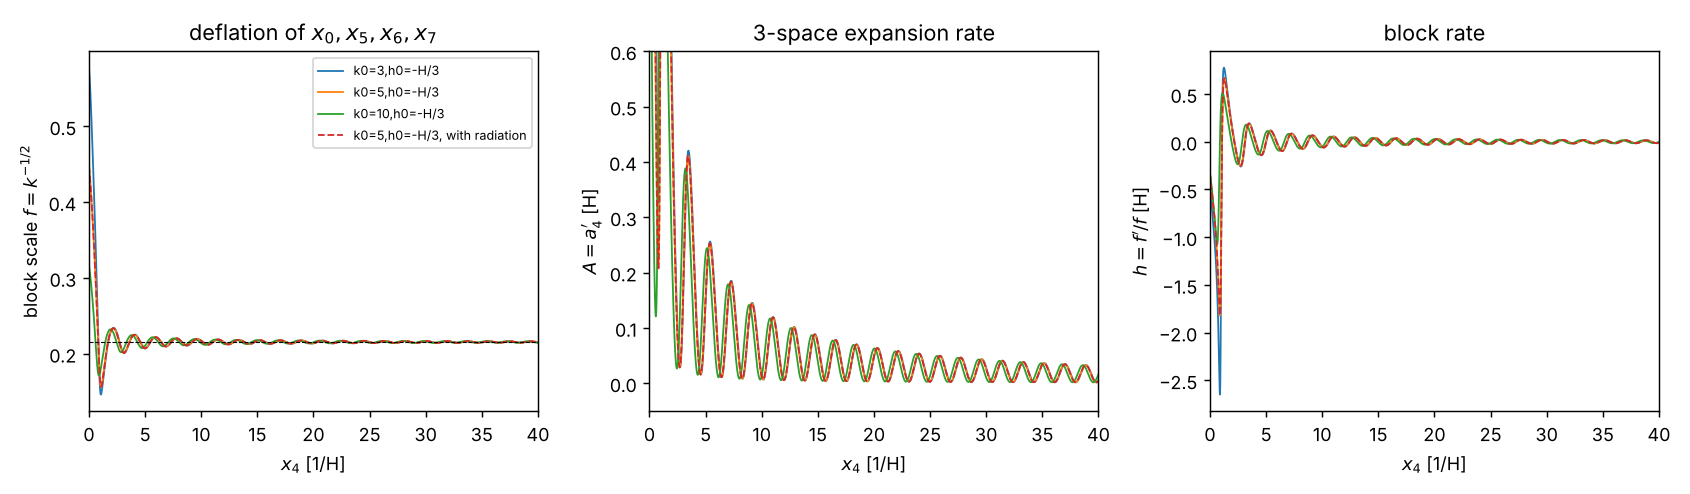
\includegraphics{figures/fig_primordial_history.png}
\caption{The primordial era: the block scale \(f\), the 3-space
expansion rate \(A\) and the block rate \(h\) for starts
\(k_0 = 3, 5, 10\) at \(h_0 = -H/3\) (one with radiation), from the full
nonlinear Einstein-Lovelock equations with the author's weights.}
\end{figure}

\hypertarget{the-response-of-the-block-to-matter-and-four-dimensional-gravity}{%
\subsection{The response of the block to matter, and four-dimensional
gravity}\label{the-response-of-the-block-to-matter-and-four-dimensional-gravity}}

To first order about the static block with block-averaged matter sources
(\(\bar p = (p_0 + 3p_t)/4\); \(A^2\) of first order,
\(3G(k_*)A^2 = \kappa\delta\rho\)) (DERIVED):
\[ \delta\ddot k + \omega_r^2\,\delta k = -2k_*\big(s_{h3}\,\kappa\delta p_3 + s_{hp}\,\kappa\delta\bar p + q_h\,\kappa\delta\rho\big),\qquad
   s_{h3} = 0.028666,\quad s_{hp} = 0.037320,\quad q_h = -0.009555;\]
the adiabatic shift is
\(\delta k = (-0.107556\,\kappa\delta p_3 - 0.140028\,\kappa\delta\bar p + 0.035852\,\kappa\delta\rho)/H^2\),
and 3-space obeys
\(\delta\dot A = -\kappa(\delta\rho + \delta p_3)/(2G(k_*))\). Together
with the constraint \(3G(k_*)A^2 = \kappa\rho\) and the dimensional
reduction
(\(\sum_p\alpha_p\mathcal L_{(p)} - 2\Lambda - 2\kappa\rho_b = G(k)R^{(4)} + \text{topological} - 2G(k)\Lambda_4\),
\(p\) the Lovelock order), the four-dimensional gravity of UM-2 is
general relativity,
\[ G^{(4)}_{\mu\nu} + \Lambda_4g_{\mu\nu} = 8\pi G_NT^{(4)}_{\mu\nu},\qquad 8\pi G_N = \frac{\kappa}{G(k_*)V_\perp},\qquad V_\perp = \frac{2f_*^4v_t(1 - e^{-3\eta})}{3H},\]
with
\(\Lambda_4 = [6H^2k(1 - 2w_2k) + \Lambda + \kappa\rho_b]/G(k) = 0\) at
the static point; the observed dark energy needs
\(\Lambda_4/H^2 \sim (H_0/H)^2 = 1.0\times10^{-92}\) (tuned; OPEN).

\hypertarget{step-2-the-masses-from-the-x_0-dependence-of-the-wave-functions}{%
\section{\texorpdfstring{Step 2: the masses from the \(x_0\) dependence
of the wave
functions}{Step 2: the masses from the x\_0 dependence of the wave functions}}\label{step-2-the-masses-from-the-x_0-dependence-of-the-wave-functions}}

Every four-dimensional mass is an eigenvalue of the \(x_0\) operator of
its field on the static block; the eigenfunctions depend on \(x_0\)
through \(y(6Hx_0)\) and are periodic with period \(\pi/(6H)\) (the
author's requirement). With \(\xi = y/L\):

\hypertarget{gauge-bosons-and-the-graviton}{%
\subsection{Gauge bosons and the
graviton}\label{gauge-bosons-and-the-graviton}}

\[ -e^{-3\eta\xi}\big(e^{3\eta\xi}u'\big)' = \Lambda u,\qquad \Lambda = (m\,fL)^2,\qquad u'(0) = 0 \text{ (even) or } u(0) = 0 \text{ (odd)},\qquad u'(-1) = \beta u(-1),\]
\[ \text{even: } \Big[q^2 + \frac{3\eta}{2}\Big(\beta + \frac{3\eta}{2}\Big)\Big]\sin q - \beta q\cos q = 0,\qquad \text{odd: } q\cos q + \Big(\beta + \frac{3\eta}{2}\Big)\sin q = 0,\qquad q^2 = \Lambda - \frac{9\eta^2}{4}.\]

\begin{longtable}[]{@{}
  >{\raggedright\arraybackslash}p{(\columnwidth - 4\tabcolsep) * \real{0.3333}}
  >{\raggedright\arraybackslash}p{(\columnwidth - 4\tabcolsep) * \real{0.3333}}
  >{\raggedright\arraybackslash}p{(\columnwidth - 4\tabcolsep) * \real{0.3333}}@{}}
\toprule\noalign{}
\begin{minipage}[b]{\linewidth}\raggedright
mode (\(\eta = 3\))
\end{minipage} & \begin{minipage}[b]{\linewidth}\raggedright
\(\Lambda = (m\,fL)^2\)
\end{minipage} & \begin{minipage}[b]{\linewidth}\raggedright
status
\end{minipage} \\
\midrule\noalign{}
\endhead
\bottomrule\noalign{}
\endlastfoot
photon, gluons, graviton (\(\beta = 0\), flat profile) & \(0\) exactly &
DERIVED \\
first even Kaluza-Klein level & \(9\eta^2/4 + \pi^2 = 30.1196\) &
DERIVED (finite elements \(1.9\times10^{-10}\)) \\
first odd level & \(27.0890\) (\(q\cot q = -9/2\)) & DERIVED (finite
elements \(4.5\times10^{-10}\)) \\
gap & \(9\eta^2/4 = 20.25\) & DERIVED \\
\(W^+\), \(W^-\) (\(\beta_W = 0.011912\)) & \(1.32149\times10^{-5}\) &
DERIVED (fit, finite elements \(3\times10^{-14}\)) \\
\(Z\) (\(\beta_Z = \beta_W/\cos^2\theta_W = 0.015343\), angle of the
couplings \(\cos^2\theta_W = (m_W^2/m_Z^2)/\rho_0 = 0.776368\)) &
\(1.70150\times10^{-5}\) & DERIVED \\
Dirichlet bound (\(\beta \to \infty\)) & \(0.010016\):
\(m_W \le 0.01824\,m_{KK}\) & DERIVED \\
\end{longtable}

Here \(\theta_W\) is the angle of the gauge couplings,
\(\cos^2\theta_W = \hat g^2/(\hat g^2 + \hat g'^2)\). The bending of the
tip-localised profiles moves the mass ratio
\(m_W^2/m_Z^2 = \Lambda_W/\Lambda_Z\) away from \(\cos^2\theta_W\), and
the electroweak parameter \(\rho = \Lambda_W/(\Lambda_Z\cos^2\theta_W)\)
exceeds 1 (\(\rho - 1 = 3.2\times10^{-8}\) at \(\beta_W = 10^{-6}\):
custodial symmetry at leading order; \(6.4\times10^{-5}\) at
\(\beta_W = 0.002\), \(3.2\times10^{-3}\) at \(0.1\)). This tree-level
custodial violation is fitted to the measured \(\rho_0 - 1 = 0.00038\)
(the violation beyond the Standard-Model loops), and the angle of the
couplings is fixed by the measured masses,
\(\rho = m_W^2/(m_Z^2\cos^2\theta_W) = \rho_0\),
i.e.~\(\cos^2\theta_W = (m_W^2/m_Z^2)/\rho_0 = 0.776368\) (on-shell
\(m_W^2/m_Z^2 = 0.776663\)); both masses are then reproduced. With
\(m_W = 80.3625\) GeV (STANDARD, PDG 2026) this gives the scales
(DERIVED)

\begin{longtable}[]{@{}
  >{\raggedright\arraybackslash}p{(\columnwidth - 2\tabcolsep) * \real{0.5000}}
  >{\raggedright\arraybackslash}p{(\columnwidth - 2\tabcolsep) * \real{0.5000}}@{}}
\toprule\noalign{}
\begin{minipage}[b]{\linewidth}\raggedright
quantity
\end{minipage} & \begin{minipage}[b]{\linewidth}\raggedright
value
\end{minipage} \\
\midrule\noalign{}
\endhead
\bottomrule\noalign{}
\endlastfoot
Kaluza-Klein mass \(m_{KK} = m_W\sqrt{\Lambda_1/\Lambda_W}\) &
\(121.32\) TeV \\
\(H = m_{KK}f_*\eta/\sqrt{\Lambda_1}\) & \(14.296\) TeV \\
proper half cell \(fL\); period of \(x_0\), \(\pi/(6H)\) &
\(8.926\times10^{-21}\) m; \(7.227\times10^{-21}\) m \\
gap \(3H/(2f_*)\) & \(99.48\) TeV \\
radion mass \(3.387H\) & \(48.42\) TeV \\
model \(m_Z = m_W\sqrt{\Lambda_Z/\Lambda_W}\) & \(91.1879\) GeV (the
measured value, reproduced) \\
\end{longtable}

\hypertarget{fermions-masses-and-mixing-of-three-generations}{%
\subsection{Fermions: masses and mixing of three
generations}\label{fermions-masses-and-mixing-of-three-generations}}

\[ h_j = j\Big[-\frac{i}{f}\sigma_1\partial_y + \mu\,\sigma_2 + e^{-a_4}k\,\sigma_3\Big],\]
with \(k\) the momentum of the mode along \(x_1\) (not the block
variable) and \(c = f\mu L\). In \(\xi = y/L\), with
\(e = \varepsilon fL\), the \(k = 0\) components \((a, b)\) of a block
\(j = +1\) obey \(a' = ca - eb\), \(b' = ea - cb\) (primes \(d/d\xi\)).
In the selected blocks of the Standard-Model fields,
\(P_{sel} = \frac{1 + \Gamma_4\gamma^{x_0}}{2}\,\frac{1 - i\gamma^{x_5}\gamma^{x_6}}{2}\),
the fold conditions \(P_{sel}(1 \mp \gamma^{x_0})\psi = 0\)
(\(\gamma^{x_0} = \sigma_3\) in block form) are \(b(0) = 0\) for a
doublet (\(c_L > 0\)) and \(a(0) = 0\) for a singlet (\(c_R < 0\)), so
that \((a_L, b_L) = (\cosh w\xi + (c_L/w)\sinh w\xi,\ (e/w)\sinh w\xi)\)
and
\((a_R, b_R) = (-(e/w)\sinh w\xi,\ \cosh w\xi - (c_R/w)\sinh w\xi)\),
and at the tip \(\xi = -1\) \((a_L, b_L) = (C_L - c_Ls_L, -s_Le)\) and
\((a_R, b_R) = (s_Re, C_R + c_Rs_R)\), \(s = \sinh w/w\),
\(C = \cosh w\), \(w = \sqrt{c^2 - e^2}\); with the tip mixing
\(b_L = \kappa_fb_R\), \(a_R = -\kappa_fa_L\) of one generation the mass
is the lowest root of
\[ D(e) = e^2s_Ls_R - \kappa_f^2(C_L - c_Ls_L)(C_R + c_Rs_R) = 0,\qquad e \simeq \kappa_f\zeta(c_L)\zeta(-c_R),\quad \zeta(c)^2 = \frac{c\,e^{-c}}{\sinh c}.\]
For three generations the tip conditions \(b_L = \kappa b_R\),
\(a_R = -\kappa^\dagger a_L\) (vectors over the generations, \(\kappa\)
the \(3\times3\) tip matrix of a sector) give, with the doublet
amplitudes \(\mathcal A\) and the singlet amplitudes \(\mathcal B\),
\[ \Big[\mathrm{diag}(b_{L\alpha}) + \kappa\,\mathrm{diag}\Big(\frac{b_{Ri}}{a_{Ri}}\Big)\kappa^\dagger\,\mathrm{diag}(a_{L\alpha})\Big]\mathcal A = 0, \]
and for a common doublet bulk mass and a unitary \(\kappa\) the
determinant is \(\prod_i(b_La_{Ri} + a_Lb_{Ri})/a_{Ri}\) with
\(b_La_R + a_Lb_R = -D(e)\vert_{\kappa_f = 1}\), the null vectors are
\(\mathcal A^{(i)} = \kappa\hat e_i\) and
\(\mathcal B^{(i)} \propto \hat e_i\): the masses are the one-generation
roots with \(\kappa_f = 1\) and the left-handed rotation of each sector
is its tip matrix, so that \(U = \kappa_e^\dagger\kappa_\nu\) and
\(V = \kappa_u^\dagger\kappa_d\) (DERIVED, \texttt{um2\_flavour.py},
mpmath with 50 digits: the roots of the \(3\times3\) determinant agree
with the one-generation roots, both refined in the same computation, to
\(3.0\times10^{-42}\) in the four sectors (the masses stored by the mass
computation agree with them to \(4.5\times10^{-11}\)), with
\(\kappa_\nu = U_{PMNS}\), \(\kappa_e = 1\), \(\kappa_u = 1\),
\(\kappa_d = V_{CKM}\), and the null vectors with the columns of
\(\kappa\) to \(1.1\times10^{-16}\); for a random complex non-unitary
tip matrix the exact roots agree with the singular values of
\(\zeta(c_L)\,\kappa\,\mathrm{diag}(\zeta(-c_{Ri}))\) to
\(3.5\times10^{-5}\), \(2.8\times10^{-6}\), \(2.0\times10^{-6}\) and the
null vectors with its left singular vectors).

With one doublet bulk mass per sector, fixed by the heaviest member with
\(c_R = -c_L\) (\(\tau\), \(t\)), the masses require (DERIVED,
\texttt{um2\_spectra.py}; exact roots; direct shooting of the coupled
\((L, R)\) Dirac system agrees with the determinant to
\(6.1\times10^{-10}\) (\(e\)), \(1.5\times10^{-11}\) (\(\tau\)),
\(5.6\times10^{-12}\) (\(t\)); the first-order formula agrees with the
exact root to the relative accuracy in the last column):

\begin{longtable}[]{@{}
  >{\raggedright\arraybackslash}p{(\columnwidth - 14\tabcolsep) * \real{0.0909}}
  >{\raggedright\arraybackslash}p{(\columnwidth - 14\tabcolsep) * \real{0.1364}}
  >{\raggedright\arraybackslash}p{(\columnwidth - 14\tabcolsep) * \real{0.1364}}
  >{\raggedright\arraybackslash}p{(\columnwidth - 14\tabcolsep) * \real{0.1364}}
  >{\raggedright\arraybackslash}p{(\columnwidth - 14\tabcolsep) * \real{0.1364}}
  >{\raggedright\arraybackslash}p{(\columnwidth - 14\tabcolsep) * \real{0.1364}}
  >{\raggedright\arraybackslash}p{(\columnwidth - 14\tabcolsep) * \real{0.1364}}
  >{\raggedright\arraybackslash}p{(\columnwidth - 14\tabcolsep) * \real{0.0909}}@{}}
\toprule\noalign{}
\begin{minipage}[b]{\linewidth}\raggedright
fermion
\end{minipage} & \begin{minipage}[b]{\linewidth}\raggedright
mass
\end{minipage} & \begin{minipage}[b]{\linewidth}\raggedright
doublet \(c\)
\end{minipage} & \begin{minipage}[b]{\linewidth}\raggedright
singlet \(c_R\)
\end{minipage} & \begin{minipage}[b]{\linewidth}\raggedright
\(\mu_R/H\)
\end{minipage} & \begin{minipage}[b]{\linewidth}\raggedright
singlet width \(fL/(2\lvert c_R\rvert)\)
\end{minipage} & \begin{minipage}[b]{\linewidth}\raggedright
\(e = m\,fL\)
\end{minipage} & \begin{minipage}[b]{\linewidth}\raggedright
first order
\end{minipage} \\
\midrule\noalign{}
\endhead
\bottomrule\noalign{}
\endlastfoot
\(\nu_1\) & \(1.000\) meV & \(5.95288\) & \(-35.04518\) & \(-54.194\) &
\(1.27\times10^{-22}\) m & \(4.5235\times10^{-17}\) &
\(5.7\times10^{-7}\) \\
\(\nu_2\) & \(8.712\) meV & \(5.95288\) & \(-32.84810\) & \(-50.796\) &
\(1.36\times10^{-22}\) m & \(3.9409\times10^{-16}\) &
\(6.1\times10^{-7}\) \\
\(\nu_3\) & \(50.140\) meV & \(5.95288\) & \(-31.07017\) & \(-48.047\) &
\(1.44\times10^{-22}\) m & \(2.2681\times10^{-15}\) &
\(6.5\times10^{-7}\) \\
\(e\) & \(0.51100\) MeV & \(5.95288\) & \(-14.55391\) & \(-22.506\) &
\(3.07\times10^{-22}\) m & \(2.3115\times10^{-8}\) &
\(1.4\times10^{-6}\) \\
\(\mu\) & \(105.658\) MeV & \(5.95288\) & \(-8.98093\) & \(-13.888\) &
\(4.97\times10^{-22}\) m & \(4.7795\times10^{-6}\) &
\(2.2\times10^{-6}\) \\
\(\tau\) & \(1776.93\) MeV & \(5.95288\) & \(-5.95288\) & \(-9.205\) &
\(7.50\times10^{-22}\) m & \(8.0380\times10^{-5}\) &
\(6.8\times10^{-6}\) \\
\(u\) & \(2.16\) MeV & \(3.38230\) & \(-15.43001\) & \(-23.861\) &
\(2.89\times10^{-22}\) m & \(9.7708\times10^{-8}\) &
\(1.3\times10^{-4}\) \\
\(c\) & \(1.2730\) GeV & \(3.38230\) & \(-8.76830\) & \(-13.559\) &
\(5.09\times10^{-22}\) m & \(5.7585\times10^{-5}\) &
\(2.2\times10^{-4}\) \\
\(t\) & \(172.56\) GeV & \(3.38230\) & \(-3.38230\) & \(-5.230\) &
\(1.32\times10^{-21}\) m & \(7.8058\times10^{-3}\) &
\(1.1\times10^{-3}\) \\
\(d\) & \(4.70\) MeV & \(3.38230\) & \(-14.62578\) & \(-22.617\) &
\(3.05\times10^{-22}\) m & \(2.1261\times10^{-7}\) &
\(1.3\times10^{-4}\) \\
\(s\) & \(93.5\) MeV & \(3.38230\) & \(-11.51582\) & \(-17.808\) &
\(3.88\times10^{-22}\) m & \(4.2295\times10^{-6}\) &
\(1.7\times10^{-4}\) \\
\(b\) & \(4.183\) GeV & \(3.38230\) & \(-7.50053\) & \(-11.599\) &
\(5.95\times10^{-22}\) m & \(1.8922\times10^{-4}\) &
\(2.6\times10^{-4}\) \\
\end{longtable}

(doublets: \(\mu_L = 9.2055\,H\), \(\mu_Q = 5.2304\,H\); the masses are
the PDG values, the light-quark masses in \(\overline{MS}\) at 2 GeV,
\(m_c(m_c)\), \(m_b(m_b)\) and the directly measured \(m_t\), used as
tree-level targets; \(m_1\) is ASSUMED, \(m_2\), \(m_3\) follow from the
NuFIT 6.0 splittings of step 5; the masses are STANDARD inputs, PDG
2025.) The mixing matrices are \(U = R_{23}U_{13}(\delta)R_{12}\) in the
standard form
\[ U = \begin{pmatrix} c_{12}c_{13} & s_{12}c_{13} & s_{13}e^{-i\delta}\\ -s_{12}c_{23} - c_{12}s_{23}s_{13}e^{i\delta} & c_{12}c_{23} - s_{12}s_{23}s_{13}e^{i\delta} & s_{23}c_{13}\\
   s_{12}s_{23} - c_{12}c_{23}s_{13}e^{i\delta} & -c_{12}s_{23} - s_{12}c_{23}s_{13}e^{i\delta} & c_{23}c_{13}\end{pmatrix},\qquad J = c_{12}s_{12}c_{23}s_{23}c_{13}^2s_{13}\sin\delta ,\]
with the NuFIT 6.0 values (\(\sin^2\theta_{12} = 0.308\),
\(\sin^2\theta_{23} = 0.470\), \(\sin^2\theta_{13} = 0.02215\),
\(\delta = 212^\circ\); \(J = -0.01777\), \(J_{max} = 0.0335\) from
these best-fit angles, against NuFIT's marginalised
\(0.0333 \pm 0.0007\)) for the PMNS matrix and the PDG values
(\(s_{12} = 0.22501\), \(s_{13} = 0.003732\), \(s_{23} = 0.04183\),
\(\delta = 1.147\); \(J = 3.117\times10^{-5}\)) for the CKM matrix, both
unitary to \(1.1\times10^{-16}\) (DERIVED). The first even Kaluza-Klein
gauge mode couples to the zero modes with the overlaps \(0.14434\)
(every left-handed lepton) and \(-0.30066\) (every left-handed quark)
relative to the zero mode, and in the mass basis its largest
off-diagonal coupling is \(1.0\times10^{-17}\): no tree-level
flavour-changing neutral current (with the three charged-lepton
\(\lvert c_R\rvert\) used as different doublet localisations it would be
\(0.033\)).
\(\mathrm{BR}(\mu\to e\gamma) = \frac{3\alpha}{32\pi}\big\lvert\sum_iU^*_{\mu i}U_{ei}m_i^2/m_W^2\big\rvert^2 = 2.8\times10^{-55}\)
(DERIVED).

\hypertarget{dirac16complex}{%
\subsection{dirac16complex}\label{dirac16complex}}

With \(M = m\), fold condition \(\chi_2(0) = 0\) (even) or
\(\chi_1(0) = 0\) (odd), tip \(\chi_2(-L) = 0\) and
\(c_\psi = f_*mL = 0.646667\), the exact \(k = 0\) spectrum is: the fold
zero mode (\(\varepsilon = 0\), all eight blocks); even bulk levels
\(\sqrt{m^2 + (n\pi/(fL))^2}\), the lowest \(4.959981\,m\); odd levels
\(\sqrt{m^2 + p^2}\) with \(\tan(p\,fL) = -p/m\), the lowest
\(3.102204\,m\) (\(p = 2.93661\,m\), \(p\,fL = 1.89901\)); and the fold
band \(\varepsilon = e^{-a_4}\lvert k\rvert\) (massless,
\(\varepsilon/\lvert k\rvert = 1\) to \(6\times10^{-14}\)) (DERIVED).

\hypertarget{step-3-kohn-sham-states-of-dirac16complex-coupled-to-all-fields}{%
\section{Step 3: Kohn-Sham states of dirac16complex coupled to all
fields}\label{step-3-kohn-sham-states-of-dirac16complex-coupled-to-all-fields}}

\hypertarget{the-kohn-sham-equations}{%
\subsection{The Kohn-Sham equations}\label{the-kohn-sham-equations}}

\[ h_j\chi_o = \varepsilon_o\chi_o,\qquad M_{eff} = m + \frac{15}{16}\lambda S + \frac{\langle\mathcal F\rangle}{\Lambda_\star^3},\qquad
   v = -\frac{\lambda}{16}n + \frac{c_V}{\Lambda_\star^6}\sum_{i=1}^3\sum_\psi q_\psi n_{\psi i},\]
\[ n = \sum wgf_on_o,\quad S = \sum wgf_os_o,\quad n_o = P\chi_o^\dagger\chi_o,\quad s_o = P\chi_o^\dagger j\sigma_2\chi_o,\quad t_o = P\chi_o^\dagger j\sigma_3\chi_o,\quad P = \frac{e^{-3Hy}}{\mathrm{Vol}_7},\]
\[ E_{KS} = \sum gf_o\varepsilon_o - 2\mathrm{Vol}_7\int e^{3Hy}e_{int}dy,\qquad e_{int} = \frac{15}{32}\lambda S^2 - \frac{1}{32}\lambda n^2,\]
\[ \rho = \sum wgf_o\varepsilon_on_o - e_{int},\qquad p_3 = \sum wgf_o\tfrac{e^{-a_4}\lvert k\rvert}{3}t_o + e_{int},\qquad p_t = e_{int},\]
\[ p_0 = \sum wgf_o[(\varepsilon_o - v)n_o - M_{eff}s_o - e^{-a_4}\lvert k\rvert t_o] + e_{int},\]
with \(w = 1/2\) per fold parity, \(g = 4r_3(\lvert\vec n\rvert^2)\) for
the momentum shell \(\vec k = \Delta k\,\vec n\)
(\(\vec n \in \mathbb Z^3\), \(r_3(\lvert\vec n\rvert^2)\) the number of
representations of \(\lvert\vec n\rvert^2\) as a sum of three squares,
\(\Delta k = 0.25\); here \(k\) is the momentum, not the block
variable), occupations \(f_o\), and
\(\mathrm{Vol}_7 = (2\pi/\Delta k)^3v_tf_*^4 = 34.27\) (\(v_t = 1\),
\(a_4 = 0\); the proper seven-volume of a cell is
\(2\,\mathrm{Vol}_7(1 - e^{-3\eta})/(3H)\)). The orbitals are expanded
in the exact free eigenfunctions of each sector (60, 120, 240 per
sector), iterated to self-consistency (tolerance \(10^{-13}\),
safeguarded Anderson mixing), and extrapolated in the basis size
(Richardson).

\hypertarget{validation}{%
\subsection{Validation}\label{validation}}

The independent solver reproduces the record's two reference states (at
\(f = 1\), \(a_4 = 0\)): \(N = 8\), \(\lambda = 157.7\):
\(E_{KS} = -0.037786682923\) (reference \(-0.037786682923\)), HOMO and
LUMO to \(10^{-14}\), integrated \(p_0 = -0.08860537545\) (reference
\(-0.08860537548\)); \(N = 592\), \(\lambda = 2.131\):
\(E_{KS} = 358.30104644787\) (identical), integrated
\(p_0 = -6.7691415097\) (reference \(-6.7691415108\)) (DERIVED).

\hypertarget{ground-states-on-the-stabilised-block}{%
\subsection{Ground states on the stabilised
block}\label{ground-states-on-the-stabilised-block}}

Two families of states (the eight \(k = 0\) fold zero modes, \(N = 8\);
a fold-band gas, \(N = 592\)) with \(\lambda = 0\), the benchmark
\(\pm\lambda_B\) (\(\lambda_B = 7\times10^{-5}H^{-6}\): mean fields
below 5 \% of \(m\)) and the record's coupling scaled to the block
(stress test, \(\lambda = 157.7f_*^4 = 0.3405\) and
\(2.131f_*^4 = 0.00460\)) (DERIVED; 120 functions per sector, relative
Richardson errors below \(2.2\times10^{-9}\)):

\begin{longtable}[]{@{}
  >{\raggedright\arraybackslash}p{(\columnwidth - 10\tabcolsep) * \real{0.1667}}
  >{\raggedright\arraybackslash}p{(\columnwidth - 10\tabcolsep) * \real{0.1667}}
  >{\raggedright\arraybackslash}p{(\columnwidth - 10\tabcolsep) * \real{0.1667}}
  >{\raggedright\arraybackslash}p{(\columnwidth - 10\tabcolsep) * \real{0.1667}}
  >{\raggedright\arraybackslash}p{(\columnwidth - 10\tabcolsep) * \real{0.1667}}
  >{\raggedright\arraybackslash}p{(\columnwidth - 10\tabcolsep) * \real{0.1667}}@{}}
\toprule\noalign{}
\begin{minipage}[b]{\linewidth}\raggedright
state
\end{minipage} & \begin{minipage}[b]{\linewidth}\raggedright
\(E_{KS}\)
\end{minipage} & \begin{minipage}[b]{\linewidth}\raggedright
\(E_{int}\)
\end{minipage} & \begin{minipage}[b]{\linewidth}\raggedright
HOMO
\end{minipage} & \begin{minipage}[b]{\linewidth}\raggedright
LUMO
\end{minipage} & \begin{minipage}[b]{\linewidth}\raggedright
iterations
\end{minipage} \\
\midrule\noalign{}
\endhead
\bottomrule\noalign{}
\endlastfoot
\(N = 8\), \(\lambda = 0\) & \(0\) & \(0\) & \(0\) & \(0.25\) & 1 \\
\(N = 8\), \(+\lambda_B\) & \(-2.053\times10^{-4}\) &
\(-2.053\times10^{-4}\) & \(-5.13\times10^{-5}\) & \(0.24995\) & 14 \\
\(N = 8\), \(-\lambda_B\) & \(2.053\times10^{-4}\) &
\(2.053\times10^{-4}\) & \(5.13\times10^{-5}\) & \(0.25005\) & 14 \\
\(N = 8\), stress & \(-0.70123\) & \(-0.42170\) & \(-0.14037\) &
\(0.10859\) & 61 \\
\(N = 592\), \(\lambda = 0\) & \(361.11614\) & \(0\) & \(0.79057\) &
\(0.82916\) & 1 \\
\(N = 592\), \(+\lambda_B\) & \(359.99060\) & \(-1.12646\) & \(0.78676\)
& \(0.82535\) & 14 \\
\(N = 592\), \(-\lambda_B\) & \(362.23906\) & \(1.12121\) & \(0.79436\)
& \(0.83295\) & 13 \\
\(N = 592\), stress & \(307.67139\) & \(-32.2217\) & \(0.64506\) &
\(0.68347\) & 56 \\
\end{longtable}

\begin{longtable}[]{@{}
  >{\raggedright\arraybackslash}p{(\columnwidth - 10\tabcolsep) * \real{0.1667}}
  >{\raggedright\arraybackslash}p{(\columnwidth - 10\tabcolsep) * \real{0.1667}}
  >{\raggedright\arraybackslash}p{(\columnwidth - 10\tabcolsep) * \real{0.1667}}
  >{\raggedright\arraybackslash}p{(\columnwidth - 10\tabcolsep) * \real{0.1667}}
  >{\raggedright\arraybackslash}p{(\columnwidth - 10\tabcolsep) * \real{0.1667}}
  >{\raggedright\arraybackslash}p{(\columnwidth - 10\tabcolsep) * \real{0.1667}}@{}}
\toprule\noalign{}
\begin{minipage}[b]{\linewidth}\raggedright
state
\end{minipage} & \begin{minipage}[b]{\linewidth}\raggedright
\(\int p_3\)
\end{minipage} & \begin{minipage}[b]{\linewidth}\raggedright
\(\int p_t\)
\end{minipage} & \begin{minipage}[b]{\linewidth}\raggedright
\(\int p_0\)
\end{minipage} & \begin{minipage}[b]{\linewidth}\raggedright
max \(\lvert\delta M\rvert\)
\end{minipage} & \begin{minipage}[b]{\linewidth}\raggedright
max \(\lvert v\rvert\)
\end{minipage} \\
\midrule\noalign{}
\endhead
\bottomrule\noalign{}
\endlastfoot
\(N = 8\), \(+\lambda_B\) & \(-2.05\times10^{-4}\) &
\(-2.05\times10^{-4}\) & \(-4.447\times10^{-4}\) & \(2.4\times10^{-7}\)
& \(6.7\times10^{-4}\) \\
\(N = 8\), \(-\lambda_B\) & \(2.05\times10^{-4}\) &
\(2.05\times10^{-4}\) & \(4.447\times10^{-4}\) & \(2.4\times10^{-7}\) &
\(6.7\times10^{-4}\) \\
\(N = 8\), stress & \(-0.4217\) & \(-0.4217\) & \(-1.30076\) & \(1.98\)
& \(1.83\) \\
\(N = 592\), \(\lambda = 0\) & \(120.372\) & \(0\) &
\(8.6\times10^{-12}\) & \(0\) & \(0\) \\
\(N = 592\), \(+\lambda_B\) & \(119.245\) & \(-1.1265\) & \(-2.43688\) &
\(1.3\times10^{-3}\) & \(0.050\) \\
\(N = 592\), \(-\lambda_B\) & \(121.493\) & \(1.1212\) & \(2.43174\) &
\(1.3\times10^{-3}\) & \(0.050\) \\
\(N = 592\), stress & \(87.614\) & \(-32.222\) & \(-97.8188\) & \(2.09\)
& \(1.88\) \\
\end{longtable}

(The integrals are \(2\mathrm{Vol}_7\int e^{3Hy}(\cdot)\,dy\); the
\(N = 8\), \(\lambda = 0\) state has all of them zero.)

Checks (DERIVED): \(E_{KS} = 2\mathrm{Vol}_7\int e^{3Hy}\rho\,dy\) to
\(4\times10^{-15}\); the \(y\)-conservation law
\([e^{3Hy}p_0]_{-L}^0 = 3H\int e^{3Hy}p_tdy\) to \(9\times10^{-8}\)
(Richardson; the raw residual falls like \(n_b^{-3}\)); observed basis
orders 4.95 (energy) and 2.97 (hidden pressure); the free gas has
\(w = \int p_3/\int\rho = 1/3\) exactly (four-dimensional radiation).
The self-interaction shifts the fold-band levels almost rigidly (the
spacing between \(k = 0\) and the first shell is \(0.25\) free,
\(0.25000\) at \(\lambda_B\), \(0.2490\) in the \(N = 8\) stress state).
A scalar mean field cannot gap the fold band at \(k = 0\):
\(\chi = (e^{f\int M_{eff}dy}, 0)\) solves
\(j[-\frac{i}{f}\sigma_1\partial_y + M_{eff}\sigma_2]\chi = 0\) with
both boundary conditions for every \(M_{eff}(y)\).

\hypertarget{dark-matter-quanta}{%
\subsection{Dark-matter quanta}\label{dark-matter-quanta}}

Eight quanta in the lowest odd level at \(k = 0\) on the \(N = 8\)
ground state add exactly \(8\varepsilon_{DM} = 24.817633063\) (computed
\(24.817633063\)) at \(\lambda = 0\) and \(24.81833\) at \(+\lambda_B\);
they are cold, \(w = p_3/\rho = 0\) (\(2.8\times10^{-5}\) with
\(\lambda_B\)); their hidden pressure is \(p_0/\rho = 0.772034343\),
equal to \(-d\ln\varepsilon_{DM}/d\ln f = 0.772034343\) obtained
independently from the \(x_0\) eigenvalue (DERIVED): the dark-matter
mass is an \(x_0\) eigenvalue, and it pushes on the block.

\hypertarget{the-standard-model-fields-acting-on-dirac16complex}{%
\subsection{The Standard-Model fields acting on
dirac16complex}\label{the-standard-model-fields-acting-on-dirac16complex}}

The portal mean fields were applied with amplitude \(e\) and shapes
given by the sources: for I11 the proper densities of the zero modes
times \(P = e^{-3Hy}/\mathrm{Vol}_7\), with the density of an
unpolarised fermion the average of its doublet and singlet zero-mode
densities, \(\varrho_c(y) = (2c/L)\,e^{2cy/L}/(1 - e^{-2c})\) for the
localisation \(c\): the electron
\(\frac12(\varrho_{c_L} + \varrho_{-c_R(e)})\) (\(c_L = 5.9529\),
\(-c_R(e) = 14.5539\)), the up quark
\(\frac12(\varrho_{c_Q} + \varrho_{-c_R(u)})\) (\(c_Q = 3.3823\),
\(-c_R(u) = 15.4300\)) and the neutrinos, produced left-chiral,
\(\varrho_{c_L}\); for I12 a uniform gluon condensate. Linear responses
of the lowest odd level (DERIVED; equal to the Hellmann-Feynman
expectation
\(d\varepsilon/de = \langle\chi\vert\partial h/\partial e\vert\chi\rangle\)
to \(10^{-8}\)):

\begin{longtable}[]{@{}
  >{\raggedright\arraybackslash}p{(\columnwidth - 4\tabcolsep) * \real{0.3333}}
  >{\raggedright\arraybackslash}p{(\columnwidth - 4\tabcolsep) * \real{0.3333}}
  >{\raggedright\arraybackslash}p{(\columnwidth - 4\tabcolsep) * \real{0.3333}}@{}}
\toprule\noalign{}
\begin{minipage}[b]{\linewidth}\raggedright
portal mean field
\end{minipage} & \begin{minipage}[b]{\linewidth}\raggedright
\(d\varepsilon_{odd}/de\)
\end{minipage} & \begin{minipage}[b]{\linewidth}\raggedright
change of the fold-band gap
\end{minipage} \\
\midrule\noalign{}
\endhead
\bottomrule\noalign{}
\endlastfoot
I11, electron density (\(v\)) & \(0.824779\) & \(5.4\times10^{-11}\) \\
I11, up-quark density (\(v\)) & \(4.328803\) & \(3.1\times10^{-9}\) \\
I11, neutrino density (\(v\), lepton doublet zero mode) & \(1.252406\) &
\(1.1\times10^{-10}\) \\
I12, gluon condensate (uniform \(M\)) & \(0.707196\) &
\(2.9\times10^{-11}\) \\
\end{longtable}

The broad quark doublet zero mode (\(c_Q = 3.38\)) overlaps the
dark-matter orbital most. The fold band stays massless under every
portal. Every orbital has \(\chi_2(-L) = 0\), so the scalar density
\(\bar\Psi\Psi = 2s_2ab\) vanishes at the tip: no tip operator built on
\(\bar\Psi\Psi\) reaches dirac16complex; the upper component does not
vanish there, so a chiral tip current would reach \(\Psi_A\) (the
projector \(P_+ = (1 - B\gamma^{x_0})/2\) annihilates every \(\Psi_B\)
orbital at the tip), but UM-2 contains none (step 4). The I12 response
defines the four-dimensional coefficient of the dark-matter operator:
\(G_i = \mathcal O\,c_ig_i^2/\Lambda_\star^3\) with
\(\mathcal O = 0.7072\).

\hypertarget{back-reaction-on-the-block}{%
\subsection{Back-reaction on the
block}\label{back-reaction-on-the-block}}

The block-averaged hidden pressure \(\bar p = (p_0 + 3p_t)/4\) of a
Kohn-Sham state displaces the block by
\(\delta k = \kappa\bar p/(3H^2 - 4\kappa\rho_b^*/k_*) = -0.140028\,\kappa\bar p/H^2\)
(stiffness \(-7.1414H^2\)), without changing the four-dimensional
cosmological term at linear order
(\(\frac{d}{dk}[6H^2k(1 - 2w_2k) + \kappa\rho_b] = -6\times10^{-12}\) at
\(k_*\)). Cell averages (units of the Kohn-Sham calculation, \(H = 1\)):
\(\bar p = -1.16\times10^{-5}\) (\(N = 8\), \(+\lambda_B\)), \(-0.0636\)
(\(N = 592\), \(+\lambda_B\)), \(\approx 0\) (free gas); the shift is
negligible for any realistic density (relative size \((A/H)^2\)). The
difference \(p_0 - p_t\) (\(-0.0574\) for \(N = 592\), \(+\lambda_B\))
drives a block-shape mode outside the order-0 metric (OPEN).

\hypertarget{step-4-the-electroweak-sector}{%
\section{Step 4: the electroweak
sector}\label{step-4-the-electroweak-sector}}

\textbf{Charges and couplings} (DERIVED): in every generation
\(Q = T_3 + Y\) gives the up-type quarks \(u\), \(c\), \(t\) the charge
\(2/3\), the down-type quarks \(d\), \(s\), \(b\) the charge \(-1/3\),
the neutrinos 0 and the charged leptons \(e\), \(\mu\), \(\tau\) the
charge \(-1\), for both chiralities; \([T_3, T_\pm] = \pm T_\pm\) with
\(Y(W) = 0\): \textbf{\(W^+ = (W^1 - iW^2)/\sqrt2\) carries \(+e\),
\(W^- = (W^1 + iW^2)/\sqrt2\) carries \(-e\)}, and \(W^-\) is the
antiparticle of \(W^+\); the photon couples with
\(e = gg'/\sqrt{g^2 + g'^2}\) times \(Q\), the \(Z\) with
\(\sqrt{g^2 + g'^2}(T_3 - Q\sin^2\theta_W)\).

\textbf{Anomalies} (DERIVED, exact fractions). With every zero mode
written as a left-handed Weyl field (\(-Y\) for a right-handed one),
\(n_c\) colours and \(n_w\) weak components, one generation gives
\[ \mathcal A_{SU(3)^2U(1)} = \sum_{\text{triplets}}n_wY = 0,\qquad \mathcal A_{SU(2)^2U(1)} = \sum_{\text{doublets}}n_cY = \tfrac12 - \tfrac12 = 0,\]
\[ \mathcal A_{U(1)^3} = \sum n_cn_wY^3 = \tfrac1{36} - \tfrac89 + \tfrac19 - \tfrac14 + 1 = 0,\]
\(\mathcal A_{grav^2U(1)} = \sum n_cn_wY = 1 - 2 + 1 - 1 + 1 = 0\) and
\(\mathcal A_{SU(3)^3} = 2 - 1 - 1 = 0\); three generations have twelve
\(SU(2)\) doublets (no Witten anomaly). Three lepton generations with a
single quark generation would leave \(\mathcal A_{SU(2)^2U(1)} = -1\)
and \(\mathcal A_{U(1)^3} = 3/2\).

\textbf{The two halves of dirac16complex.} \(B\) commutes with the
four-dimensional Lorentz generators and with \(C\), so
\(\Psi = \Psi_A + \Psi_B\) (\(B = -1\), \(B = +1\)) splits into
Lorentz-invariant halves and
\(\bar\Psi\Psi = \bar\Psi_A\Psi_A + \bar\Psi_B\Psi_B\); the identity
\(\Gamma_4 = -B\gamma^{x_0}\) (DERIVED, \(16\times16\)) gives
\(P_+ = (1 + \Gamma_4)/2 = (1 - B\gamma^{x_0})/2\), which equals
\((1 + \gamma^{x_0})/2\) on \(\Psi_A\) and \((1 - \gamma^{x_0})/2\) on
\(\Psi_B\); the latter annihilates every orbital at the tip. The chiral
charge densities \(u^\dagger P_+u\) at the tip (what a chiral tip
current would couple to) are (DERIVED): \(\Psi_A\) fold band
\(a_0(-L)^2 = 0.163\) per unit length in each of its four blocks,
\(\Psi_B\) fold band \(0\); \(\Psi_A\) odd (heavy) states \(0.257\),
\(\Psi_B\) odd states \(0\); every transition current
\(\bar\Psi_A\gamma^\mu P_+\Psi_B\) vanishes at the tip.

\textbf{The \(Z\) invisible width and the tip \(Z\) portal of version
1.} Version 1 coupled the \(\Psi_A\) fold band (two Weyl species) to the
\(Z\) through the chiral tip portal
\(S_{I9} = \int_{y=-L}d^7x\sqrt{\lvert g_{tip}\rvert}\,(c_Z + c'_Z\varsigma)(i\bar\Psi\gamma^\mu P_+\Psi)\,\frac{iv_\Sigma^2}{2}\mathrm{tr}(\Sigma^\dagger D_\mu\Sigma\tau^3)\)
(\(\varsigma = \pm1\) the side of the tip). With three neutrinos and a
fold-band coupling \(r\) times a neutrino's,
\[ N_\nu = \frac{\Gamma_{inv}}{\Gamma(Z\to\nu\bar\nu)} = 3 + 2r^2 ;\]
the measured \(N_\nu = 2.9963 \pm 0.0074\) (PDG 2025) is reproduced by
\(r = 0\) (0.5 standard deviations) and bounds \(r^2 < 0.0056\) (two
standard deviations). Even at that bound the neutral-current rate of the
fold band, \(r^2\) times the neutrino's (\(\propto r^2G_F^2T^5\) against
\(H \propto T^2/M_{Pl}\)), keeps it in equilibrium down to
\(T \approx 2.6\,\text{MeV}\times r^{-2/3} = 14.7\) MeV, where
\(g_s = 10.75\), so it would carry the neutrino temperature and add
\[ \Delta N_{eff} = n_W\Big(\frac{10.75}{g_s}\Big)^{4/3}F_h,\qquad F_h = \Big[\frac{T_\nu}{T_\gamma}\Big(\frac{11}{4}\Big)^{1/3}\Big/(1 + h_\nu)\Big]^4 = 1.0095 \]
(\(n_W = 2\) Weyl species; \(F_h\) corrects for the non-instantaneous
neutrino decoupling of step 5, \(T_\nu/T_\gamma = 0.71664\) and the
comoving heating \(h_\nu = 0.00165\) with one common temperature: a
species decoupled earlier is not heated by \(e^+e^-\) annihilation),
\(\Delta N_{eff} = 2.02\), far above the measured
\(N_{eff} = 2.99 \pm 0.17\) (Planck 2018) and \(2.86 \pm 0.13\) (ACT
DR6) (STANDARD). The oriented part \(c'_Z\) (odd under the fold
reflection) would let the heavy odd \(\Psi_A\) states decay,
\(\Psi_A^{odd} \to \Psi_A^{fold} + Z\), and through the inverse decays
and the exchange process \(\Psi_A^{fold}Z \to \Psi_A^{fold}Z\) keep the
fold band in equilibrium until the odd states disappear,
\(T \sim M_{DM}/30\) (above the electroweak scale, \(g_s = 105.75\): the
Standard Model without a Higgs particle), or, for \(c'_Z\) of the size
of a neutrino's coupling, until the \(Z\) bosons annihilate near 15 GeV
(\(g_s = 86.25\): \(t\), \(W\), \(Z\) gone) (ESTIMATE): then
\(\Delta N_{eff} = 0.0958\) to \(0.1257\) and \(N_{eff} = 3.139\) to
\(3.169\), \(2.1\) to \(2.4\) standard deviations above ACT DR6 (the
three-flavour value \(3.0432\): \(1.4\); disfavoured). UM-2 therefore
drops the portal, \(c_Z = c'_Z = 0\) (ASSUMED; the bounds DERIVED,
\texttt{um2\_electroweak.py}): \(N_\nu = 3\), neither fold band is ever
thermalised, and both halves keep an exact fold parity. (For reference,
the plasma counts used are \(g_s = 10.75\): photons, \(e^\pm\), three
neutrinos; \(61.75\) just above the QCD crossover: \(+\) gluons, \(u\),
\(d\), \(s\), \(\mu\); \(86.25\) below the top, \(W\) and \(Z\) masses;
\(105.75\) above the electroweak scale. Right-handed neutrinos are never
thermalised.)

\textbf{The \(Z\) widths of three generations} (tree level, massless
fermions;
\(\Gamma(Z \to f\bar f) = N_cG_Fm_Z^3(g_V^2 + g_A^2)/(6\sqrt2\pi)\),
\(g_V = T_3 - 2Q\sin^2\theta_W\) with the \(\overline{MS}\) value
\(\sin^2\theta_W = 0.23122\), \(g_A = T_3\); \(G_F\), \(m_Z\) and the
\(\overline{MS}\) angle STANDARD; DERIVED):

\begin{longtable}[]{@{}
  >{\raggedright\arraybackslash}p{(\columnwidth - 14\tabcolsep) * \real{0.1250}}
  >{\raggedright\arraybackslash}p{(\columnwidth - 14\tabcolsep) * \real{0.1250}}
  >{\raggedright\arraybackslash}p{(\columnwidth - 14\tabcolsep) * \real{0.1250}}
  >{\raggedright\arraybackslash}p{(\columnwidth - 14\tabcolsep) * \real{0.1250}}
  >{\raggedright\arraybackslash}p{(\columnwidth - 14\tabcolsep) * \real{0.1250}}
  >{\raggedright\arraybackslash}p{(\columnwidth - 14\tabcolsep) * \real{0.1250}}
  >{\raggedright\arraybackslash}p{(\columnwidth - 14\tabcolsep) * \real{0.1250}}
  >{\raggedright\arraybackslash}p{(\columnwidth - 14\tabcolsep) * \real{0.1250}}@{}}
\toprule\noalign{}
\begin{minipage}[b]{\linewidth}\raggedright
channel
\end{minipage} & \begin{minipage}[b]{\linewidth}\raggedright
each \(\nu\)
\end{minipage} & \begin{minipage}[b]{\linewidth}\raggedright
invisible (\(3\nu\))
\end{minipage} & \begin{minipage}[b]{\linewidth}\raggedright
each of \(e\), \(\mu\), \(\tau\)
\end{minipage} & \begin{minipage}[b]{\linewidth}\raggedright
each of \(u\), \(c\)
\end{minipage} & \begin{minipage}[b]{\linewidth}\raggedright
each of \(d\), \(s\), \(b\)
\end{minipage} & \begin{minipage}[b]{\linewidth}\raggedright
hadronic
\end{minipage} & \begin{minipage}[b]{\linewidth}\raggedright
total
\end{minipage} \\
\midrule\noalign{}
\endhead
\bottomrule\noalign{}
\endlastfoot
tree level (MeV) & \(165.9\) & \(497.7\) & \(83.4\) & \(285.4\) &
\(367.9\) & \(1674.4\) & \(2422.3\) \\
with \(1 + \alpha_s/\pi\) on the quarks (MeV) & & & & & & \(1737.3\) &
\(2485.2\) \\
measured (PDG 2025, MeV) & & \(499.1\) & & & & & \(2495.5\) \\
\end{longtable}

The top quark is too heavy for the \(Z\) to decay into it;
\(\alpha_s(m_Z) = 0.1180\) (STANDARD). The ratio
\(R_\ell = \Gamma_{had}/\Gamma_{\ell\ell} = 20.83\) compares with the
measured \(20.77\) (STANDARD, PDG 2025). The remaining differences
(\(0.4\) \% in the total) are the size of the electroweak loop
corrections, which UM-2 does not compute; with the tree-level angle of
the couplings of the mass fit, \(\sin^2\theta_W = 0.22363\), the total
changes by \(+0.82\) \% (a per-cent scheme ambiguity). The
one-generation conflict of version 1 (a total of \(1232\) MeV) is gone.

\hypertarget{step-5-the-flavour-conversion-of-the-three-neutrinos}{%
\section{Step 5: the flavour conversion of the three
neutrinos}\label{step-5-the-flavour-conversion-of-the-three-neutrinos}}

\hypertarget{masses-mixing-and-the-equations}{%
\subsection{Masses, mixing and the
equations}\label{masses-mixing-and-the-equations}}

The neutrino masses are the \(x_0\) eigenvalues of step 2 with the
lightest mass chosen (ASSUMED) and the normal ordering (the NuFIT 6.0
best fit; the inverted ordering has \(\Delta\chi^2 = 6.1\)):
\[ m_1 = 1.000\ \text{meV},\qquad m_2 = \sqrt{m_1^2 + \Delta m^2_{21}} = 8.712\ \text{meV},\qquad m_3 = \sqrt{m_1^2 + \Delta m^2_{31}} = 50.140\ \text{meV}, \]
\(\Delta m^2_{21} = 7.49\times10^{-5}\) eV\(^2\),
\(\Delta m^2_{31} = 2.513\times10^{-3}\) eV\(^2\);
\(\sum m_\nu = 0.0599\) eV, below the DESI DR2 bound \(0.064\) eV
(DERIVED, \texttt{um2\_neutrino.py}, 15 checks). The PMNS matrix is the
neutrino tip matrix of step 2. The flavour amplitudes \(\psi_\alpha\) of
a neutrino of energy \(E\) evolve with
\[ i\frac{d\psi}{dx_4} = \mathcal H\psi,\qquad \mathcal H = \frac{1}{2E}\,U\,\mathrm{diag}(m_1^2, m_2^2, m_3^2)\,U^\dagger + \mathrm{diag}(V_{CC}, 0, 0),\qquad V_{CC} = \sqrt2\,G_Fn_e \]
(the flavour-universal neutral-current potential drops out;
antineutrinos: \(U \to U^*\), \(V_{CC} \to -V_{CC}\)), solved exactly by
\(S = e^{-i\mathcal HL}\) for a constant density and by the ordered
product of layer operators otherwise, with
\(P(\nu_\alpha\to\nu_\beta) = \lvert S_{\beta\alpha}\rvert^2\). In
vacuum
\[ P(\nu_\alpha\to\nu_\beta) = \Big\lvert\sum_iU_{\beta i}U^*_{\alpha i}e^{-im_i^2L/(2E)}\Big\rvert^2,\]
\[ P(\nu_\mu\to\nu_e) - P(\nu_e\to\nu_\mu) = -16J\sin\Delta_{21}\sin\Delta_{31}\sin\Delta_{32},\qquad \Delta_{ij} = \frac{\Delta m^2_{ij}L}{4E}. \]

\hypertarget{vacuum-matter-and-accelerators}{%
\subsection{Vacuum, matter and
accelerators}\label{vacuum-matter-and-accelerators}}

Checks (DERIVED): the exact evolution reproduces the vacuum formula to
\(3.9\times10^{-15}\), unitarity to \(1.8\times10^{-15}\), CPT
(\(P(\nu_\alpha\to\nu_\beta) = \bar P(\bar\nu_\beta\to\bar\nu_\alpha)\))
to \(2.8\times10^{-16}\) and the T-odd difference to
\(5.9\times10^{-14}\) at reactor, accelerator and atmospheric baselines.
Reactor \(\bar\nu_e\) of 4 MeV survive with \(\bar P_{ee} = 0.9183\) at
1.65 km, \(0.2263\) at 52.5 km and \(0.2674\) at 180 km; the vacuum
\(\nu_\mu\) survival has its first minimum, \(0.0060\), at
\(L/E = 1516\) km/GeV. The 1-3 MSW resonance,
\(2EV_{CC} = \Delta m^2_{ee}\cos2\theta_{13}\) with
\(\Delta m^2_{ee} = c_{12}^2\Delta m^2_{31} + s_{12}^2\Delta m^2_{32}\),
lies at \(11.135\) GeV for \(\rho = 2.8\) g/cm\(^3\), \(Y_e = 0.5\)
(\(n_e = \rho Y_eN_A\)); the exact three-flavour Hamiltonian has
\(\lvert U^m_{e3}\rvert^2 = 1/2\) at \(11.133\) GeV (agreement
\(1.6\times10^{-4}\); with \(\Delta m^2_{31}\) alone the formula gives
\(11.24\) GeV). The 1-2 resonance at the centre of the Sun
(\(n_e = 100N_A\) cm\(^{-3}\)),
\(2EV_{CC}c_{13}^2 = \Delta m^2_{21}\cos2\theta_{12}\), lies at \(1.93\)
MeV. Long-baseline appearance in matter of constant density
(\(\delta = 212^\circ\), normal ordering):

\begin{longtable}[]{@{}
  >{\raggedright\arraybackslash}p{(\columnwidth - 14\tabcolsep) * \real{0.1250}}
  >{\raggedright\arraybackslash}p{(\columnwidth - 14\tabcolsep) * \real{0.1250}}
  >{\raggedright\arraybackslash}p{(\columnwidth - 14\tabcolsep) * \real{0.1250}}
  >{\raggedright\arraybackslash}p{(\columnwidth - 14\tabcolsep) * \real{0.1250}}
  >{\raggedright\arraybackslash}p{(\columnwidth - 14\tabcolsep) * \real{0.1250}}
  >{\raggedright\arraybackslash}p{(\columnwidth - 14\tabcolsep) * \real{0.1250}}
  >{\raggedright\arraybackslash}p{(\columnwidth - 14\tabcolsep) * \real{0.1250}}
  >{\raggedright\arraybackslash}p{(\columnwidth - 14\tabcolsep) * \real{0.1250}}@{}}
\toprule\noalign{}
\begin{minipage}[b]{\linewidth}\raggedright
experiment
\end{minipage} & \begin{minipage}[b]{\linewidth}\raggedright
\(L\) (km)
\end{minipage} & \begin{minipage}[b]{\linewidth}\raggedright
\(E\) (GeV)
\end{minipage} & \begin{minipage}[b]{\linewidth}\raggedright
\(\rho\) (g/cm\(^3\))
\end{minipage} & \begin{minipage}[b]{\linewidth}\raggedright
\(P(\nu_\mu\to\nu_e)\)
\end{minipage} & \begin{minipage}[b]{\linewidth}\raggedright
\(\bar P(\bar\nu_\mu\to\bar\nu_e)\)
\end{minipage} & \begin{minipage}[b]{\linewidth}\raggedright
vacuum \(P(\nu_\mu\to\nu_e)\)
\end{minipage} & \begin{minipage}[b]{\linewidth}\raggedright
\(P(\nu_\mu\to\nu_\mu)\)
\end{minipage} \\
\midrule\noalign{}
\endhead
\bottomrule\noalign{}
\endlastfoot
T2K & 295 & 0.6 & 2.6 & \(0.0517\) & \(0.0313\) & \(0.0478\) &
\(0.0085\) \\
NOvA & 810 & 2.0 & 2.84 & \(0.0481\) & \(0.0236\) & \(0.0404\) &
\(0.1010\) \\
DUNE & 1300 & 2.5 & 2.848 & \(0.0701\) & \(0.0195\) & \(0.0491\) &
\(0.0098\) \\
\end{longtable}

The matter effect raises the neutrino and lowers the antineutrino
appearance for the normal ordering, and the phase \(\delta = 212^\circ\)
adds to the asymmetry.

\hypertarget{the-sun}{%
\subsection{The Sun}\label{the-sun}}

With the electron density
\(n_e(r) = N_A\min(245\,e^{-10.54\,r/R_\odot}, 100)\) cm\(^{-3}\)
(ASSUMED profile) and production at the radius \(r_0\), the adiabatic
survival probability is
\[ P_{ee} = c_{13}^4\Big(\frac12 + \frac12\cos2\theta_{12}\cos2\theta^m_{12}(r_0)\Big) + s_{13}^4,\qquad
   \cos2\theta^m_{12} = \frac{\cos2\theta_{12} - A}{\sqrt{(\cos2\theta_{12} - A)^2 + \sin^22\theta_{12}}},\qquad A = \frac{2EV_{CC}(r_0)c_{13}^2}{\Delta m^2_{21}}, \]
and the numerical three-flavour evolution through 20000 and 40000 layers
from \(r_0\) to the surface, followed by the incoherent sum over the
mass states, \(P_{ee} = \sum_i\lvert U_{ei}\rvert^2P(\nu_i)\), gives
(DERIVED):

\begin{longtable}[]{@{}
  >{\raggedright\arraybackslash}p{(\columnwidth - 8\tabcolsep) * \real{0.2000}}
  >{\raggedright\arraybackslash}p{(\columnwidth - 8\tabcolsep) * \real{0.2000}}
  >{\raggedright\arraybackslash}p{(\columnwidth - 8\tabcolsep) * \real{0.2000}}
  >{\raggedright\arraybackslash}p{(\columnwidth - 8\tabcolsep) * \real{0.2000}}
  >{\raggedright\arraybackslash}p{(\columnwidth - 8\tabcolsep) * \real{0.2000}}@{}}
\toprule\noalign{}
\begin{minipage}[b]{\linewidth}\raggedright
source
\end{minipage} & \begin{minipage}[b]{\linewidth}\raggedright
\(E\) (MeV)
\end{minipage} & \begin{minipage}[b]{\linewidth}\raggedright
\(r_0/R_\odot\)
\end{minipage} & \begin{minipage}[b]{\linewidth}\raggedright
\(P_{ee}\) adiabatic
\end{minipage} & \begin{minipage}[b]{\linewidth}\raggedright
\(P_{ee}\) numerical
\end{minipage} \\
\midrule\noalign{}
\endhead
\bottomrule\noalign{}
\endlastfoot
pp & 0.30 & 0.10 & \(0.5409\) & \(0.5408\) \\
\(^7\)Be & 0.862 & 0.06 & \(0.5197\) & \(0.5196\) \\
pep & 1.44 & 0.07 & \(0.4978\) & \(0.4976\) \\
\(^8\)B & 5.0 & 0.05 & \(0.3771\) & \(0.3767\) \\
\(^8\)B & 10.0 & 0.05 & \(0.3194\) & \(0.3185\) \\
\(^8\)B & 15.0 & 0.05 & \(0.3055\) & \(0.3043\) \\
\end{longtable}

The two agree to \(1.3\times10^{-3}\) (the layer convergence is
\(2.2\times10^{-6}\)): the conversion is adiabatic, vacuum dominated at
low energy
(\(P_{ee} \to c_{13}^4(1 - \frac12\sin^22\theta_{12}) + s_{13}^4\)) and
matter dominated for \(^8\)B
(\(P_{ee} \to c_{13}^4\sin^2\theta_{12} + s_{13}^4\)).

\begin{figure}
\centering
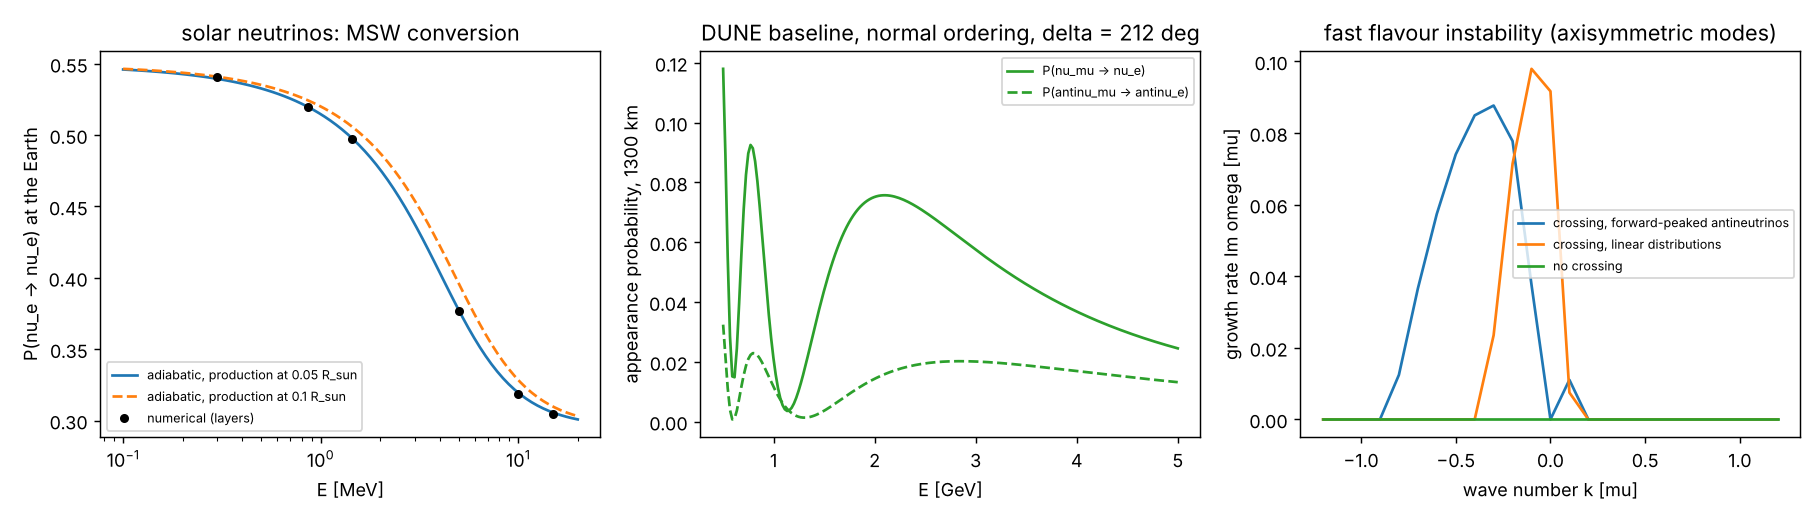
\includegraphics{figures/fig_neutrino_conversion.png}
\caption{Flavour conversion in UM-2. Left: the solar \(\nu_e\) survival
probability (adiabatic formula for two production radii, numerical
evolution as points). Middle: \(\nu_\mu\to\nu_e\) and
\(\bar\nu_\mu\to\bar\nu_e\) appearance over 1300 km of rock (normal
ordering, \(\delta = 212^\circ\)). Right: the growth rate of the fast
flavour instability against the wave number for the three angular
distributions of the text.}
\end{figure}

\hypertarget{the-early-universe-and-n_eff}{%
\subsection{\texorpdfstring{The early Universe and
\(N_{eff}\)}{The early Universe and N\_\{eff\}}}\label{the-early-universe-and-n_eff}}

The thermal potential of the \(e^\pm\) plasma,
\[ V_e - V_\mu = -\frac{8\sqrt2\,G_Fp}{3m_W^2}\,\frac{7\pi^2}{60}T^4 , \]
falls below \(\Delta m^2\cos2\theta/(2p)\) at the mean momentum
\(p = 3.15T\) when \(T = 4.99\) MeV for the atmospheric and \(T = 2.39\)
MeV for the solar splitting (DERIVED; \(m_W\) of the UM-2 fit): the
flavours mix while the neutrinos decouple. The decoupling is computed
from the temperature equations (Escudero's method; MeV units, the Hubble
rate \(H = \sqrt{8\pi\rho/3}/M_{Pl}\), \(M_{Pl} = 1.22091\times10^{19}\)
GeV)
\[ \frac{dT_\gamma}{dx_4} = -\frac{4H\rho_\gamma + 3H(\rho_e + p_e) + 3HT_\gamma\frac{dP_{int}}{dT_\gamma} + \frac{\delta\rho_{\nu_e}}{\delta x_4} + 2\frac{\delta\rho_{\nu_\mu}}{\delta x_4}}
   {\frac{d\rho_\gamma}{dT_\gamma} + \frac{d\rho_e}{dT_\gamma} + T_\gamma\frac{d^2P_{int}}{dT_\gamma^2}},\qquad
   \frac{dT_{\nu_\alpha}}{dx_4} = -HT_{\nu_\alpha} + \frac{\delta\rho_{\nu_\alpha}/\delta x_4}{d\rho_{\nu_\alpha}/dT_{\nu_\alpha}}, \]
\[ \frac{\delta\rho_{\nu_e}}{\delta x_4} = \frac{G_F^2}{\pi^5}\Big[4(g_{eL}^2 + g_{eR}^2)F(T_\gamma, T_{\nu_e}) + 2F(T_{\nu_\mu}, T_{\nu_e})\Big],\qquad
   \frac{\delta\rho_{\nu_\mu}}{\delta x_4} = \frac{G_F^2}{\pi^5}\Big[4(g_{\mu L}^2 + g_{\mu R}^2)F(T_\gamma, T_{\nu_\mu}) - F(T_{\nu_\mu}, T_{\nu_e})\Big], \]
\[ F(T_1, T_2) = 32f_a(T_1^9 - T_2^9) + 56f_sT_1^4T_2^4(T_1 - T_2),\qquad f_a = 0.884,\quad f_s = 0.829, \]
with \(\rho_\gamma = \pi^2T_\gamma^4/15\),
\(\rho_{\nu_\alpha} = 7\pi^2T_{\nu_\alpha}^4/120\) per flavour
(\(\nu_\tau\) as \(\nu_\mu\)), the \(e^\pm\) density and pressure with
the electron mass, the effective couplings \(g_{eL} = 0.727\),
\(g_{eR} = 0.233\), \(g_{\mu L} = -0.273\), \(g_{\mu R} = 0.233\) (or
the UM-2 tree-level couplings \(\frac12 + s^2\), \(s^2\),
\(-\frac12 + s^2\), \(s^2\), \(s^2 = 0.22363\)), and the QED interaction
pressure \(P_{int} = P_2 + P_3\),
\[ P_2 = -\frac{e^2T^2}{12\pi^2}J_1 - \frac{e^2}{8\pi^4}J_1^2 + \frac{e^2m_e^2}{16\pi^4}J_2,\qquad P_3 = \frac{e^3T}{12\pi^4}I^{3/2},\qquad \rho_{int} = -P_{int} + T\frac{dP_{int}}{dT}, \]
\[ J_1 = \int_0^\infty dp\,\frac{p^2}{E}n_D,\qquad J_2 = \int_0^\infty\!\!\int_0^\infty dp\,dq\,\frac{pq}{E_pE_q}\ln\Big\lvert\frac{p + q}{p - q}\Big\rvert n_D(p)n_D(q),\qquad
   I = \int_0^\infty dp\,\frac{p^2 + E^2}{E}n_D, \]
\(n_D = 2/(e^{E/T} + 1)\), \(E = \sqrt{p^2 + m_e^2}\). The integrals are
evaluated with Gauss-Legendre panels; the logarithmic singularity of
\(J_2\) at \(q = p\) is removed by the substitution \(q = p(1 - s^2)\),
and the massless limits \(P_2 = -5e^2T^4/288\),
\(P_3 = e^3T^4/(36\sqrt3\pi)\), \(\rho_e = 7\pi^2T^4/60\) are reproduced
to \(10^{-16}\). The equations run from \(T = 20\) MeV to \(5\) keV
(LSODA, relative tolerance \(10^{-11}\)), and
\[ N_{eff} = \Big(\frac{11}{4}\Big)^{4/3}\Big[\Big(\frac{T_{\nu_e}}{T_\gamma}\Big)^4 + 2\Big(\frac{T_{\nu_\mu}}{T_\gamma}\Big)^4\Big]; \]
for instantaneous decoupling at \(T_d = 20\) MeV the plasma entropy
\(a^3(\rho + p)/T\) (with \(\rho_{int}\), \(P_{int}\)) is conserved and
\(T_\nu \propto 1/a\). Results (DERIVED):

\begin{longtable}[]{@{}
  >{\raggedright\arraybackslash}p{(\columnwidth - 4\tabcolsep) * \real{0.3333}}
  >{\raggedright\arraybackslash}p{(\columnwidth - 4\tabcolsep) * \real{0.3333}}
  >{\raggedright\arraybackslash}p{(\columnwidth - 4\tabcolsep) * \real{0.3333}}@{}}
\toprule\noalign{}
\begin{minipage}[b]{\linewidth}\raggedright
run
\end{minipage} & \begin{minipage}[b]{\linewidth}\raggedright
\(N_{eff}\)
\end{minipage} & \begin{minipage}[b]{\linewidth}\raggedright
published (Escudero 2020, same method, Table 1 there)
\end{minipage} \\
\midrule\noalign{}
\endhead
\bottomrule\noalign{}
\endlastfoot
instantaneous decoupling, no QED & \(3.0002\) & \(3.000\) \\
instantaneous, \(O(e^2)\) QED & \(3.0108\) & \(3.011\) \\
instantaneous, \(O(e^2) + O(e^3)\) & \(3.0098\) & \(3.010\) \\
Fermi-Dirac energy transfer, one neutrino temperature, no QED &
\(3.0393\) & \(3.039\) \\
the same with \(O(e^2)\) & \(3.0495\) & \\
the same with \(O(e^2) + O(e^3)\) & \(3.0485\) & \(3.049\) \\
UM-2, separate \(\nu_e\) and \(\nu_{\mu,\tau}\) temperatures (no
oscillations), \(O(e^3)\) & \(3.0476\) & \(3.048\) (separate
temperatures) \\
UM-2, separate temperatures, UM-2 tree-level couplings & \(3.0472\) & \\
UM-2, one common temperature (efficient oscillations) & \(3.0485\) & \\
\end{longtable}

With separate temperatures \(T_{\nu_e}/T_\gamma = 0.71732\) and
\(T_{\nu_\mu}/T_\gamma = 0.71621\); \(e^+e^-\) annihilation raises the
comoving neutrino temperatures by \(0.265\) \% (\(\nu_e\), which also
has charged-current interactions with the electrons) and \(0.109\) \%
(\(\nu_{\mu,\tau}\)). The plasma of UM-2 at MeV temperatures is that of
the three-flavour Standard Model and contains no extra radiation, so the
precision Standard-Model value with oscillations and the electron mass
in the rates is adopted:
\[ N_{eff} = 3.0432 \pm 0.0002\qquad \text{(Cielo, Escudero, Mangano and Pisanti 2023)}, \]
from which the computed range \(3.0476\) to \(3.0485\) differs by
\(0.0044\) to \(0.0053\) (the remaining difference is the electron mass
in the rates and the momentum dependence, which the method of
temperatures does not resolve).

\begin{figure}
\centering
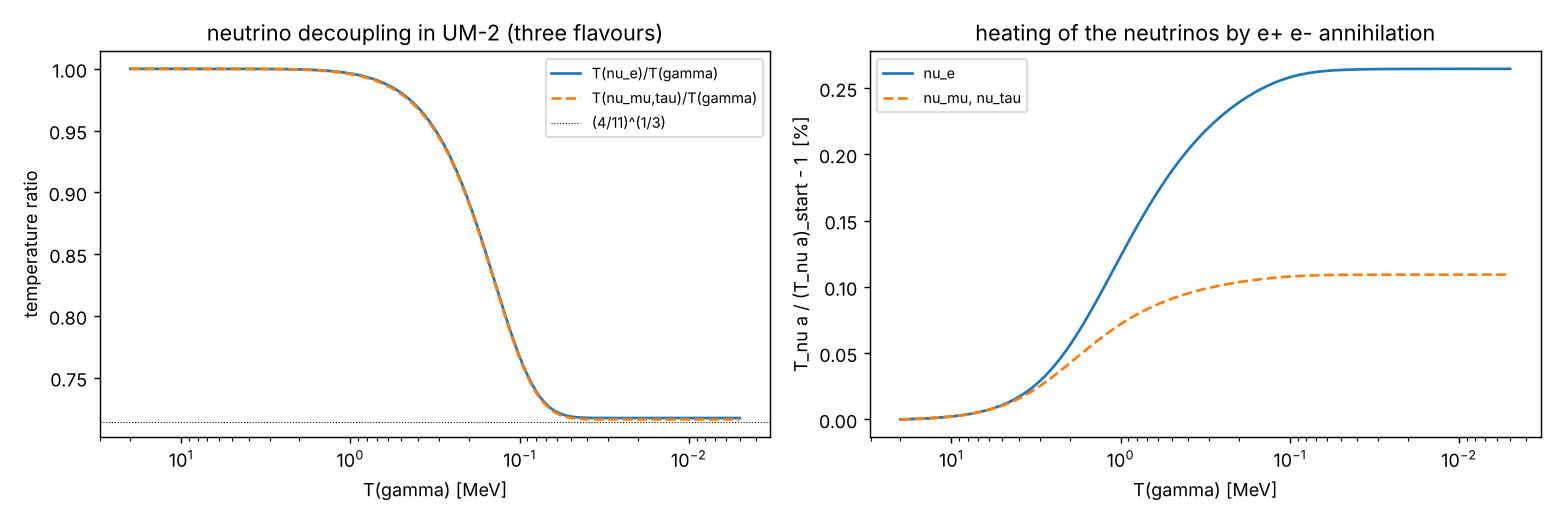
\includegraphics{figures/fig_neutrino_decoupling.png}
\caption{Neutrino decoupling in UM-2 (three flavours, separate \(\nu_e\)
and \(\nu_{\mu,\tau}\) temperatures, QED to \(O(e^3)\)). Left: the
neutrino temperatures relative to the photon temperature; right: the
comoving heating of the neutrinos by \(e^+e^-\) annihilation.}
\end{figure}

\hypertarget{the-cosmic-neutrino-background}{%
\subsection{The cosmic neutrino
background}\label{the-cosmic-neutrino-background}}

After decoupling the flavour coherence is lost: the CNB of UM-2 is an
incoherent mixture of the three mass eigenstates with the Fermi-Dirac
spectrum \(f = 1/(e^{p/T_\nu} + 1)\) (\(T_{CMB} = 2.7255\) K, STANDARD),
\[ T_\nu = \Big(\frac{4}{11}\Big)^{1/3}T_{CMB} = 1.9454\ \text{K} = 1.676\times10^{-4}\ \text{eV},\qquad n_i = \frac{3\zeta(3)}{2\pi^2}T_\nu^3 = 112.0\ \text{cm}^{-3}\ (\nu_i + \bar\nu_i), \]
\[ \rho_i = 2\int\frac{d^3p}{(2\pi)^3}\sqrt{p^2 + m_i^2}\,f,\qquad \Omega_\nu h^2 = \frac{\sum_i\rho_i}{\rho_c/h^2} = 6.382\times10^{-4}\quad (\rho_c/h^2 = 1.05368\times10^4\ \text{eV/cm}^3), \]
compared with the non-relativistic value
\(\sum m_i/94.06\ \text{eV} = 6.363\times10^{-4}\) at this temperature
(the semi-relativistic \(\nu_1\), whose energy density exceeds
\(m_1n_1\) by 16 \%, adds \(0.3\) \%), with the conventional
\(\sum m_i/93.14\ \text{eV} = 6.426\times10^{-4}\) (which includes the
heating of the non-instantaneous decoupling) and with
\(6.451\times10^{-4}\) for the heated spectrum of \(N_{eff} = 3.0432\)
(step 6: the degeneracy \(N_{eff}/3\) of each state corresponds to a
Fermi-Dirac spectrum of temperature \((N_{eff}/3)^{1/4}T_\nu\), so the
non-relativistic density is multiplied by \((N_{eff}/3)^{3/4}\)). The
states (DERIVED; mean velocity
\(\langle v\rangle = \int p^2(p/E)f\,dp/\int p^2f\,dp\),
\(E = \sqrt{p^2 + m_i^2}\)):

\begin{longtable}[]{@{}
  >{\raggedright\arraybackslash}p{(\columnwidth - 12\tabcolsep) * \real{0.1000}}
  >{\raggedright\arraybackslash}p{(\columnwidth - 12\tabcolsep) * \real{0.1500}}
  >{\raggedright\arraybackslash}p{(\columnwidth - 12\tabcolsep) * \real{0.1500}}
  >{\raggedright\arraybackslash}p{(\columnwidth - 12\tabcolsep) * \real{0.1500}}
  >{\raggedright\arraybackslash}p{(\columnwidth - 12\tabcolsep) * \real{0.1500}}
  >{\raggedright\arraybackslash}p{(\columnwidth - 12\tabcolsep) * \real{0.1500}}
  >{\raggedright\arraybackslash}p{(\columnwidth - 12\tabcolsep) * \real{0.1500}}@{}}
\toprule\noalign{}
\begin{minipage}[b]{\linewidth}\raggedright
state
\end{minipage} & \begin{minipage}[b]{\linewidth}\raggedright
mass (meV)
\end{minipage} & \begin{minipage}[b]{\linewidth}\raggedright
\(n\) (cm\(^{-3}\))
\end{minipage} & \begin{minipage}[b]{\linewidth}\raggedright
\(\langle v\rangle/c\) today
\end{minipage} & \begin{minipage}[b]{\linewidth}\raggedright
\(\lvert U_{ei}\rvert^2\)
\end{minipage} & \begin{minipage}[b]{\linewidth}\raggedright
\(\lvert U_{\mu i}\rvert^2\)
\end{minipage} & \begin{minipage}[b]{\linewidth}\raggedright
\(\lvert U_{\tau i}\rvert^2\)
\end{minipage} \\
\midrule\noalign{}
\endhead
\bottomrule\noalign{}
\endlastfoot
\(\nu_1\) & \(1.000\) & \(112.0\) & \(0.435\) & \(0.677\) & \(0.112\) &
\(0.211\) \\
\(\nu_2\) & \(8.712\) & \(112.0\) & \(0.0604\) & \(0.301\) & \(0.428\) &
\(0.271\) \\
\(\nu_3\) & \(50.140\) & \(112.0\) & \(0.0105\) & \(0.022\) & \(0.460\)
& \(0.518\) \\
\end{longtable}

The fold bands of dirac16complex are not part of the CNB (they are never
thermalised, step 4).

\hypertarget{supernovae}{%
\subsection{Supernovae}\label{supernovae}}

\textbf{The MSW resonances of the envelope.} With
\(\rho(r) = 10^4\,(10^9\,\text{cm}/r)^3\) g/cm\(^3\), \(Y_e = 0.5\)
(ASSUMED), a resonance lies at
\(n_e = \Delta m^2\cos2\theta/(2\sqrt2\,G_FE)\), i.e.~at \(r\) with
\(d\ln n_e/dr = -3/r\), its adiabaticity is
\(\gamma = \Delta m^2\sin^22\theta/(2E\cos2\theta\,\lvert d\ln n_e/dr\rvert)\)
and the jump probability \(P_{LZ} = e^{-\pi\gamma/2}\) (DERIVED;
two-flavour conditions: \(\Delta m^2_{31}\) and \(\theta_{13}\) for the
H resonance, \(\Delta m^2_{21}\) and \(\theta_{12}\) for the L
resonance, without the factor \(c_{13}^2\) of the solar condition, which
would move the L densities by 2 \%, and without \(\Delta m^2_{ee}\),
which would move the H densities by 1 \%):

\begin{longtable}[]{@{}
  >{\raggedright\arraybackslash}p{(\columnwidth - 12\tabcolsep) * \real{0.1000}}
  >{\raggedright\arraybackslash}p{(\columnwidth - 12\tabcolsep) * \real{0.2000}}
  >{\raggedright\arraybackslash}p{(\columnwidth - 12\tabcolsep) * \real{0.1500}}
  >{\raggedright\arraybackslash}p{(\columnwidth - 12\tabcolsep) * \real{0.1000}}
  >{\raggedright\arraybackslash}p{(\columnwidth - 12\tabcolsep) * \real{0.2000}}
  >{\raggedright\arraybackslash}p{(\columnwidth - 12\tabcolsep) * \real{0.1500}}
  >{\raggedright\arraybackslash}p{(\columnwidth - 12\tabcolsep) * \real{0.1000}}@{}}
\toprule\noalign{}
\begin{minipage}[b]{\linewidth}\raggedright
\(E\) (MeV)
\end{minipage} & \begin{minipage}[b]{\linewidth}\raggedright
H (1-3): \(\rho_{res}\) (g/cm\(^3\))
\end{minipage} & \begin{minipage}[b]{\linewidth}\raggedright
\(r_{res}\) (km)
\end{minipage} & \begin{minipage}[b]{\linewidth}\raggedright
\(\gamma\)
\end{minipage} & \begin{minipage}[b]{\linewidth}\raggedright
L (1-2): \(\rho_{res}\) (g/cm\(^3\))
\end{minipage} & \begin{minipage}[b]{\linewidth}\raggedright
\(r_{res}\) (km)
\end{minipage} & \begin{minipage}[b]{\linewidth}\raggedright
\(\gamma\)
\end{minipage} \\
\midrule\noalign{}
\endhead
\bottomrule\noalign{}
\endlastfoot
10 & \(3147\) & \(1.47\times10^4\) & \(283\) & \(37.7\) &
\(6.43\times10^4\) & \(903\) \\
20 & \(1573\) & \(1.85\times10^4\) & \(178\) & \(18.8\) &
\(8.10\times10^4\) & \(569\) \\
40 & \(787\) & \(2.33\times10^4\) & \(112\) & \(9.42\) &
\(1.02\times10^5\) & \(358\) \\
\end{longtable}

Both resonances are adiabatic (\(P_{LZ} \le 2.6\times10^{-77}\)). For
the normal ordering a \(\nu_e\) produced in the core leaves the star as
\(\nu_3\), \(P(\nu_e\to\nu_e) = \lvert U_{e3}\rvert^2 = 0.02215\), and
an \(\bar\nu_e\) as \(\bar\nu_1\),
\(\bar P(\bar\nu_e\to\bar\nu_e) = \lvert U_{e1}\rvert^2 = 0.677\)
(without collective effects and Earth matter). For representative
accretion-phase neutrinospheres (\(L = 6\), \(6\), \(4\times10^{52}\)
erg/s and \(\langle E\rangle = 11\), \(14\), \(15.5\) MeV for \(\nu_e\),
\(\bar\nu_e\), \(\nu_x\); ASSUMED), number fluxes
\(N \propto L/\langle E\rangle\) and the survival probabilities \(P\),
\(\bar P\) above, the mean energies observed at the Earth,
\[ \langle E\rangle_{\nu_e} = \frac{PN_e\langle E\rangle_e + (1 - P)N_x\langle E\rangle_x}{PN_e + (1 - P)N_x},\qquad
   \langle E\rangle_{\bar\nu_e} = \frac{\bar PN_{\bar e}\langle E\rangle_{\bar e} + (1 - \bar P)N_x\langle E\rangle_x}{\bar PN_{\bar e} + (1 - \bar P)N_x}, \]
become \(15.29\) MeV (\(\nu_e\)) and \(14.34\) MeV (\(\bar\nu_e\)).

\textbf{The fast flavour instability.} With the ELN distribution
\(G(u) = \sqrt2G_F[n_{\nu_e}g_{\nu_e}(u) - n_{\bar\nu_e}g_{\bar\nu_e}(u)]\)
in units of \(\mu = \sqrt2G_Fn_{\nu_e}\)
(\(G/\mu = g_{\nu_e} - \alpha g_{\bar\nu_e}\),
\(\alpha = n_{\bar\nu_e}/n_{\nu_e}\)), the dispersion relation of the
linearised equations for modes \(e^{-i(\Omega x_4 - Kx_3)}\) along the
symmetry axis \(x_3\), \(\det\Pi = 0\) with
\(\Pi^{\mu\nu} = \eta^{\mu\nu} + \int du/2\,G\,v^\mu v^\nu/(\omega - ku)\),
\(v = (1, u)\), \(\eta^{\mu\nu} = \mathrm{diag}(1, -1)\) on
\((x_4, x_3)\), has the axisymmetric branch
\((1 + J_0)(-1 + J_2) - J_1^2 = 0\),
\(J_n = \int du/2\,G\,u^n/(\omega - ku)\), and the azimuthal branch
\(-1 + \int du/2\,G(1 - u^2)/(2(\omega - ku)) = 0\)
(\(\omega = \Omega - \Lambda^0\), \(k = K - \Lambda^3\),
\(\Lambda^\mu = \int du/2\,G\,v^\mu\)). The roots with
\(\mathrm{Im}\,\omega > 0\) were found for real \(k\) on a grid
(\(-1.2 \le k \le 1.2\), step \(0.1\)) by vectorised Newton iterations
with the analytic derivative from a grid of complex starting points
(DERIVED):

\begin{longtable}[]{@{}
  >{\raggedright\arraybackslash}p{(\columnwidth - 8\tabcolsep) * \real{0.2000}}
  >{\raggedright\arraybackslash}p{(\columnwidth - 8\tabcolsep) * \real{0.2000}}
  >{\raggedright\arraybackslash}p{(\columnwidth - 8\tabcolsep) * \real{0.2000}}
  >{\raggedright\arraybackslash}p{(\columnwidth - 8\tabcolsep) * \real{0.2000}}
  >{\raggedright\arraybackslash}p{(\columnwidth - 8\tabcolsep) * \real{0.2000}}@{}}
\toprule\noalign{}
\begin{minipage}[b]{\linewidth}\raggedright
angular distributions
\end{minipage} & \begin{minipage}[b]{\linewidth}\raggedright
ELN crossing
\end{minipage} & \begin{minipage}[b]{\linewidth}\raggedright
largest growth (branch, \(k\))
\end{minipage} & \begin{minipage}[b]{\linewidth}\raggedright
homogeneous mode
\end{minipage} & \begin{minipage}[b]{\linewidth}\raggedright
mode \(K = \Lambda^3\)
\end{minipage} \\
\midrule\noalign{}
\endhead
\bottomrule\noalign{}
\endlastfoot
\(g_{\nu_e} \propto e^{-(1-u)^2/(2\cdot0.6^2)}\),
\(g_{\bar\nu_e} \propto e^{-(1-u)^2/(2\cdot0.4^2)}\), \(\alpha = 0.8\) &
yes & \(0.0877\,\mu\) (axisymmetric, \(k = -0.30\)) & \(0.0185\,\mu\) &
stable \\
\(g_{\nu_e} = 1 + 0.2u\), \(g_{\bar\nu_e} = 1 + 0.6u\), \(\alpha = 0.9\)
& yes & \(0.0979\,\mu\) (axisymmetric, \(k = -0.10\)) & stable &
\(0.0917\,\mu\) \\
as the first, \(\alpha = 0.3\) & no & none & stable & stable \\
\end{longtable}

(the largest azimuthal growth rates are \(0.0200\,\mu\) and
\(0.0050\,\mu\) for the first two cases). Three independent evaluations
agree to \(1.2\times10^{-14}\): the analytic growth
\(\frac12\sqrt{4I_1^2 - (I_0 + I_2)^2}\) (\(I_n = \int du/2\,G\,u^n\))
of the mode \(K = \Lambda^3\) against the root of the dispersion
relation at \(k = 0\), and the eigenvalues of the discretised
homogeneous equations
\(i\,dS_u/dx_4 = (\Lambda^0 - u\Lambda^3)S_u - \int du'/2\,G(u')(1 - uu')S_{u'}\)
(300 nodes) against the root at \(k = -\Lambda^3\). With an ELN crossing
the gas is unstable, without one it is not, as Morinaga's theorem (2022)
states; the second case shows that a stable homogeneous mode does not
exclude growing inhomogeneous modes. Near the neutrinosphere,
\(n_{\nu_e} = 10^{32}\) to \(10^{33}\) cm\(^{-3}\)
(\(\mu = 1.27\times10^{-5}\) to \(1.27\times10^{-4}\) eV), the first
case grows by \(e\) in \(5.9\times10^{-10}\) to \(5.9\times10^{-11}\) s
over \(17.8\) to \(1.78\) cm: a million times faster than the
hydrodynamics, which is why explosion models treat the conversion as
instantaneous.

\textbf{Flavour conversion and the explosions.} The charged-current
heating behind the shock is, schematically,
\(q \propto N_e\langle E^2\rangle_e + N_{\bar e}\langle E^2\rangle_{\bar e}\)
with \(\langle E^2\rangle = \frac54\langle E\rangle^2\) (spectra with
the pinching parameter 3). Full three-flavour equipartition gives
\(q' = \frac13(N_e\langle E^2\rangle_e + 2N_x\langle E^2\rangle_x) + \frac13(N_{\bar e}\langle E^2\rangle_{\bar e} + 2N_x\langle E^2\rangle_x)\),
and pair conversion \(\nu_e\bar\nu_e \to \nu_x\bar\nu_x\) of
\(\Delta = \frac23(N_{\bar e} - N_x)\) pairs, which conserves the ELN
until \(\bar\nu_e\) is equipartitioned,
\(q'' = (1 - \Delta/N_e)N_e\langle E^2\rangle_e + (1 - \Delta/N_{\bar e})N_{\bar e}\langle E^2\rangle_{\bar e}\);
for the neutrinospheres above \(q'/q = 0.884\) and \(q''/q = 0.760\)
(DERIVED, schematic): the heavy-lepton neutrinos are more energetic but
fewer and do not heat through charged currents. Gogilashvili and
Tamborra (2026, arXiv:2605.16504) simulated 195 progenitors of 9 to 120
solar masses (GR1D, M1 transport of \(\nu_e\), \(\bar\nu_e\), \(\nu_x\)
in 18 energy bins, SFHo equation of state) with instantaneous flavour
equipartition, conserving the electron lepton number and the number and
momentum of the neutrinos in each energy bin, imposed at 0.02 s after
bounce where the baryon density is below \(\rho_c\) (STANDARD, cited):

\begin{longtable}[]{@{}
  >{\raggedright\arraybackslash}p{(\columnwidth - 10\tabcolsep) * \real{0.1667}}
  >{\raggedright\arraybackslash}p{(\columnwidth - 10\tabcolsep) * \real{0.1667}}
  >{\raggedright\arraybackslash}p{(\columnwidth - 10\tabcolsep) * \real{0.1667}}
  >{\raggedright\arraybackslash}p{(\columnwidth - 10\tabcolsep) * \real{0.1667}}
  >{\raggedright\arraybackslash}p{(\columnwidth - 10\tabcolsep) * \real{0.1667}}
  >{\raggedright\arraybackslash}p{(\columnwidth - 10\tabcolsep) * \real{0.1667}}@{}}
\toprule\noalign{}
\begin{minipage}[b]{\linewidth}\raggedright
\(\rho_c\) (g/cm\(^3\))
\end{minipage} & \begin{minipage}[b]{\linewidth}\raggedright
no conversion
\end{minipage} & \begin{minipage}[b]{\linewidth}\raggedright
\(10^9\)
\end{minipage} & \begin{minipage}[b]{\linewidth}\raggedright
\(10^{10}\)
\end{minipage} & \begin{minipage}[b]{\linewidth}\raggedright
\(10^{11}\)
\end{minipage} & \begin{minipage}[b]{\linewidth}\raggedright
\(10^{13}\)
\end{minipage} \\
\midrule\noalign{}
\endhead
\bottomrule\noalign{}
\endlastfoot
failed explosions & \(25.6\) \% & \(50.8\) \% & \(77.4\) \% & \(93.3\)
\% & \(96.4\) \% \\
weighted with the Salpeter mass function & \(27.0\) \% & \(47.6\) \% &
\(61.9\) \% & \(73.9\) \% & \(88.3\) \% \\
\end{longtable}

The effect is strongest between 16 and 30 solar masses (easing the
red-supergiant and supernova-rate problems), and the successful
explosions leave lighter neutron stars (gravitational masses around 1.2
to 1.4 solar masses); the authors caution that the large fractions for
deep conversion are in tension with observations and call for dynamical,
multi-dimensional treatments.

\hypertarget{step-6-the-cmb-the-cnb-and-the-bao}{%
\section{Step 6: the CMB, the CNB and the
BAO}\label{step-6-the-cmb-the-cnb-and-the-bao}}

The four-dimensional effective theory is general relativity (step 1)
with photons, baryons, the three neutrino mass eigenstates, the dark
matter (the odd quanta of \(\Psi_A\) and \(\Psi_B\)) and \(\Lambda_4\);
there is no dark radiation. Its linear perturbations obey the standard
Einstein-Boltzmann equations (Newtonian gauge, conformal time,
\(ds^2 = a^2[-(1 + 2\psi)d\tau^2 + (1 - 2\phi)d\vec x^{\,2}]\)):
\[ k^2\phi + 3\mathcal H(\phi' + \mathcal H\psi) = -4\pi G_Na^2\delta\rho,\qquad k^2(\phi' + \mathcal H\psi) = 4\pi G_Na^2(\bar\rho + \bar P)\theta,\]
\[ \phi'' + \mathcal H(\psi' + 2\phi') + (2\mathcal H' + \mathcal H^2)\psi + \frac{k^2}{3}(\phi - \psi) = 4\pi G_Na^2\delta P,\qquad k^2(\phi - \psi) = 12\pi G_Na^2(\bar\rho + \bar P)\sigma,\]
with the cold dark matter \(\delta_c' = -\theta_c + 3\phi'\),
\(\theta_c' = -\mathcal H\theta_c + k^2\psi\); the baryons and photons
coupled by Thomson scattering (\(n_e\) the free-electron density,
\(\sigma_T\) the Thomson cross-section,
\(R = 4\bar\rho_\gamma/(3\bar\rho_b)\), \(c_s\) the baryon sound speed,
\(F_{\gamma l}\) and \(G_{\gamma l}\) the temperature and polarisation
multipoles, \(F_{\gamma2} = 2\sigma_\gamma\)),
\[ \delta_b' = -\theta_b + 3\phi',\qquad \theta_b' = -\mathcal H\theta_b + c_s^2k^2\delta_b + R\,an_e\sigma_T(\theta_\gamma - \theta_b) + k^2\psi, \]
\[ \delta_\gamma' = -\tfrac43\theta_\gamma + 4\phi',\qquad \theta_\gamma' = k^2\big(\tfrac14\delta_\gamma - \sigma_\gamma\big) + k^2\psi + an_e\sigma_T(\theta_b - \theta_\gamma), \]
\[ F_{\gamma l}' = \frac{k}{2l + 1}\big[lF_{\gamma(l-1)} - (l + 1)F_{\gamma(l+1)}\big] - an_e\sigma_T\Big[F_{\gamma l} - \frac{\delta_{l2}}{10}\big(F_{\gamma2} + G_{\gamma0} + G_{\gamma2}\big)\Big]\quad (l \ge 2),\]
\[ G_{\gamma l}' = \frac{k}{2l + 1}\big[lG_{\gamma(l-1)} - (l + 1)G_{\gamma(l+1)}\big] + an_e\sigma_T\Big[-G_{\gamma l} + \frac12\big(F_{\gamma2} + G_{\gamma0} + G_{\gamma2}\big)\Big(\delta_{l0} + \frac{\delta_{l2}}{5}\Big)\Big] ;\]
and one massive hierarchy per neutrino mass state \(i\) (comoving
momentum \(q\), energy \(E_i = \sqrt{q^2 + a^2m_i^2}\), multipoles
\(\mathcal N^{(i)}_l\) of the perturbed Fermi-Dirac distribution
\(\bar f_\nu\)):
\(\mathcal N^{(i)\prime}_0 = -\frac{qk}{E_i}\mathcal N^{(i)}_1 - \phi'\frac{d\ln\bar f_\nu}{d\ln q}\),
\(\mathcal N^{(i)\prime}_1 = \frac{qk}{3E_i}(\mathcal N^{(i)}_0 - 2\mathcal N^{(i)}_2) - \frac{E_ik}{3q}\psi\frac{d\ln\bar f_\nu}{d\ln q}\),
\(\mathcal N^{(i)\prime}_l = \frac{qk}{(2l+1)E_i}[l\mathcal N^{(i)}_{l-1} - (l+1)\mathcal N^{(i)}_{l+1}]\)
(\(l \ge 2\)). They were solved with CAMB 2.0.5 at the Planck 2018
values (STANDARD) \(\omega_b = 0.02237\), \(\omega_c = 0.1200\),
\(100\theta_{MC} = 1.04092\), \(\tau_{reio} = 0.0544\) (the optical
depth to reionisation), \(\ln(10^{10}A_s) = 3.044\), \(n_s = 0.9649\)
(\(\theta\) held fixed, so \(H_0\) is an output; \(H_0\) in km/s/Mpc).
In UM-2 the three mass states are evolved separately, each with the
degeneracy \(N_{eff}/3 = 1.0144\) (the heated spectrum); CAMB gives each
the density \(\deg\times\rho_{FD}(m'; T_\nu)\) at
\(T_\nu = (4/11)^{1/3}T_{CMB}\), so its masses are
\(m'_i = m_i\deg^{-1/4}\), which reproduce the late-time density
\(m_in_\nu\deg^{3/4}\) of the heated spectrum; CAMB finds \(m'_i\) by
inverting the full (relativistic) density from \(\omega_\nu\) and the
mass fractions, which were therefore iterated (13 iterations) until the
masses agree to \(7.8\times10^{-12}\) (DERIVED). The models are
\(\Lambda\)CDM with the Planck 2018 parameters (one neutrino of \(0.06\)
eV, \(N_{eff} = 3.044\): the CAMB defaults), UM-2, and two variants with
a thermalised fold band of dirac16complex (two Weyl species, which UM-2
does not contain; step 4), decoupled above the electroweak scale
(\(\Delta N_{eff} = 0.0958\)) or just above the QCD crossover
(\(\Delta N_{eff} = 2(10.75/61.75)^{4/3}\times1.0095 = 0.1963\))
(DERIVED, \texttt{um2\_cosmology.py}, 6 checks). The BAO distances
\(D_M(z) = \int_0^z c\,dz'/H(z')\) (flat), \(D_H = c/H(z)\),
\(D_V = (zD_M^2D_H)^{1/3}\), in units of the drag-epoch sound horizon
\(r_d\), are compared with the DESI DR2 measurements (STANDARD,
arXiv:2503.14738)

\begin{longtable}[]{@{}
  >{\raggedright\arraybackslash}p{(\columnwidth - 10\tabcolsep) * \real{0.1667}}
  >{\raggedright\arraybackslash}p{(\columnwidth - 10\tabcolsep) * \real{0.1667}}
  >{\raggedright\arraybackslash}p{(\columnwidth - 10\tabcolsep) * \real{0.1667}}
  >{\raggedright\arraybackslash}p{(\columnwidth - 10\tabcolsep) * \real{0.1667}}
  >{\raggedright\arraybackslash}p{(\columnwidth - 10\tabcolsep) * \real{0.1667}}
  >{\raggedright\arraybackslash}p{(\columnwidth - 10\tabcolsep) * \real{0.1667}}@{}}
\toprule\noalign{}
\begin{minipage}[b]{\linewidth}\raggedright
tracer
\end{minipage} & \begin{minipage}[b]{\linewidth}\raggedright
\(z\)
\end{minipage} & \begin{minipage}[b]{\linewidth}\raggedright
\(D_V/r_d\)
\end{minipage} & \begin{minipage}[b]{\linewidth}\raggedright
\(D_M/r_d\)
\end{minipage} & \begin{minipage}[b]{\linewidth}\raggedright
\(D_H/r_d\)
\end{minipage} & \begin{minipage}[b]{\linewidth}\raggedright
\(r_{MH}\)
\end{minipage} \\
\midrule\noalign{}
\endhead
\bottomrule\noalign{}
\endlastfoot
BGS & 0.295 & \(7.942 \pm 0.075\) & & & \\
LRG1 & 0.510 & & \(13.588 \pm 0.167\) & \(21.863 \pm 0.425\) &
\(-0.459\) \\
LRG2 & 0.706 & & \(17.351 \pm 0.177\) & \(19.455 \pm 0.330\) &
\(-0.404\) \\
LRG3+ELG1 & 0.934 & & \(21.576 \pm 0.152\) & \(17.641 \pm 0.193\) &
\(-0.416\) \\
ELG2 & 1.321 & & \(27.601 \pm 0.318\) & \(14.176 \pm 0.221\) &
\(-0.434\) \\
QSO & 1.484 & & \(30.512 \pm 0.760\) & \(12.817 \pm 0.516\) &
\(-0.500\) \\
Ly\(\alpha\) & 2.330 & & \(38.988 \pm 0.531\) & \(8.632 \pm 0.101\) &
\(-0.431\) \\
\end{longtable}

through \(\chi^2 = \sum_i(d_i - d_i^{th})^TC_i^{-1}(d_i - d_i^{th})\),
\(C_i = \begin{pmatrix}\sigma_M^2 & r_{MH}\sigma_M\sigma_H\\ r_{MH}\sigma_M\sigma_H & \sigma_H^2\end{pmatrix}\),
for the pairs \(d_i = (D_M/r_d, D_H/r_d)\) of the anisotropic tracers
(\(d_i^{th}\) the computed pair) and \((d - d^{th})^2/\sigma_V^2\) for
BGS:

\begin{longtable}[]{@{}
  >{\raggedright\arraybackslash}p{(\columnwidth - 16\tabcolsep) * \real{0.1111}}
  >{\raggedright\arraybackslash}p{(\columnwidth - 16\tabcolsep) * \real{0.1111}}
  >{\raggedright\arraybackslash}p{(\columnwidth - 16\tabcolsep) * \real{0.1111}}
  >{\raggedright\arraybackslash}p{(\columnwidth - 16\tabcolsep) * \real{0.1111}}
  >{\raggedright\arraybackslash}p{(\columnwidth - 16\tabcolsep) * \real{0.1111}}
  >{\raggedright\arraybackslash}p{(\columnwidth - 16\tabcolsep) * \real{0.1111}}
  >{\raggedright\arraybackslash}p{(\columnwidth - 16\tabcolsep) * \real{0.1111}}
  >{\raggedright\arraybackslash}p{(\columnwidth - 16\tabcolsep) * \real{0.1111}}
  >{\raggedright\arraybackslash}p{(\columnwidth - 16\tabcolsep) * \real{0.1111}}@{}}
\toprule\noalign{}
\begin{minipage}[b]{\linewidth}\raggedright
model
\end{minipage} & \begin{minipage}[b]{\linewidth}\raggedright
\(H_0\)
\end{minipage} & \begin{minipage}[b]{\linewidth}\raggedright
\(\Omega_m\)
\end{minipage} & \begin{minipage}[b]{\linewidth}\raggedright
\(N_{eff}\)
\end{minipage} & \begin{minipage}[b]{\linewidth}\raggedright
\(Y_{He}\)
\end{minipage} & \begin{minipage}[b]{\linewidth}\raggedright
age (Gyr)
\end{minipage} & \begin{minipage}[b]{\linewidth}\raggedright
\(z_*\)
\end{minipage} & \begin{minipage}[b]{\linewidth}\raggedright
\(r_{drag}\) (Mpc)
\end{minipage} & \begin{minipage}[b]{\linewidth}\raggedright
BAO \(\chi^2\) (13 points)
\end{minipage} \\
\midrule\noalign{}
\endhead
\bottomrule\noalign{}
\endlastfoot
\(\Lambda\)CDM & \(67.34\) & \(0.3154\) & \(3.044\) & \(0.24566\) &
\(13.799\) & \(1089.91\) & \(147.103\) & \(32.55\) \\
UM-2 & \(67.37\) & \(0.3151\) & \(3.0432\) & \(0.24566\) & \(13.797\) &
\(1089.91\) & \(147.109\) & \(31.72\) \\
UM-2 + fold band (electroweak) & \(68.48\) & \(0.3050\) & \(3.1390\) &
\(0.24693\) & \(13.698\) & \(1090.00\) & \(146.630\) & \(15.43\) \\
UM-2 + fold band (QCD) & \(69.65\) & \(0.2948\) & \(3.2395\) &
\(0.24824\) & \(13.596\) & \(1090.10\) & \(146.133\) & \(10.65\) \\
\end{longtable}

\(\Omega_\nu h^2 = 6.4511\times10^{-4}\) in CAMB, equal to
\(6.4510\times10^{-4}\) from the CNB of step 5 times
\((N_{eff}/3)^{3/4}\); the mass sum \(0.0599\) eV lies below the DESI
DR2 bound \(0.064\) eV, which would allow \(m_1 < 4.1\) meV. The UM-2 TT
and EE spectra agree with Planck \(\Lambda\)CDM to \(2.8\times10^{-4}\)
(\(30 \le \ell \le 2500\); for TT at most \(0.007\) of the cosmic
variance \(\sqrt{2/(2\ell + 1)}\) of a single multipole; the binned
full-sky cosmic-variance \(\chi^2 = \sum_b(\bar\delta_b/\sigma_b)^2\)
over bins \(b\) of \(\Delta\ell = 50\), with \(\bar\delta_b\) the mean
relative deviation and
\(\sigma_b = \sqrt{2/\sum_{\ell\in b}(2\ell + 1)}\), is \(0.023\)): UM-2
reproduces the CMB of \(\Lambda\)CDM. By themselves the three mass
states instead of one state of 60 meV move TT and EE by
\(2.6\times10^{-4}\) and \(2.3\times10^{-4}\), and \(N_{eff} = 3.0432\)
instead of \(3.044\) by \(1.3\times10^{-4}\). The fold-band variants, at
fixed Planck \(\omega_b\), \(\omega_c\), \(\theta_*\), move TT by up to
\(1.5\) \% and \(3.1\) \% (\(0.8\) and \(1.5\) cosmic-variance units of
a single multipole; binned \(\chi^2 = 293\) and \(1208\)): they are not
fits to the CMB, and they lie \(2.1\) and \(2.9\) standard deviations
above the ACT DR6 value \(N_{eff} = 2.86 \pm 0.13\) (UM-2: \(1.4\)). The
CNB enters through \(N_{eff} = 3.0432\) and the three neutrino masses.

\begin{figure}
\centering
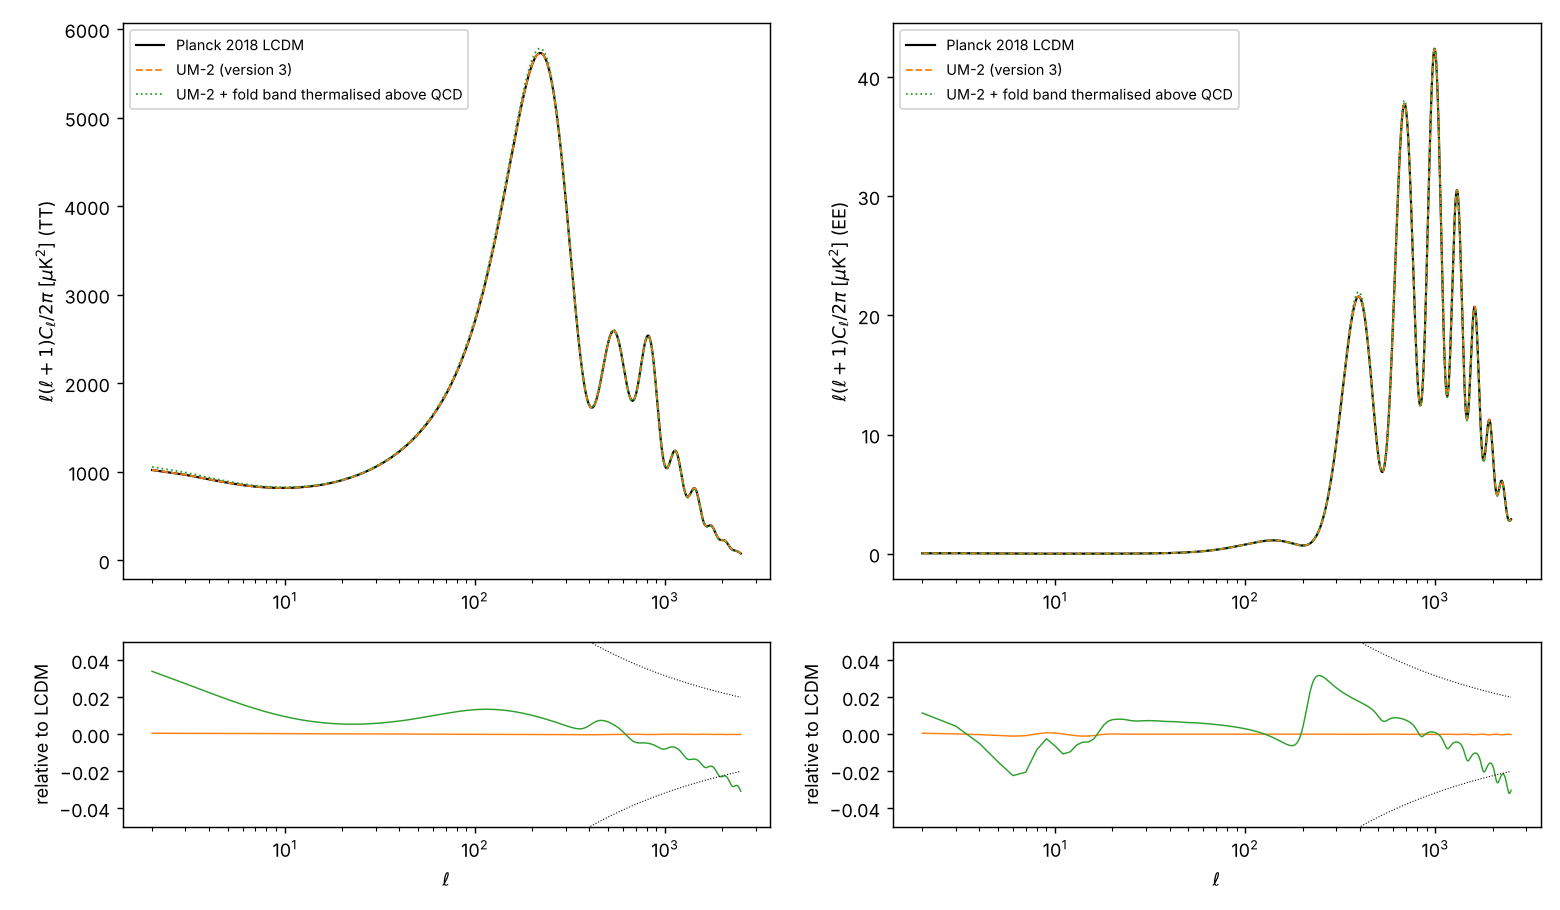
\includegraphics{figures/fig_cmb_spectra.png}
\caption{CMB temperature (left) and E-mode (right) spectra of UM-2
(three massive neutrinos), of Planck 2018 \(\Lambda\)CDM and of the
variant with a fold band thermalised above the QCD crossover; lower
panels: relative difference to \(\Lambda\)CDM with the cosmic variance
of one multipole (dotted).}
\end{figure}

\begin{figure}
\centering
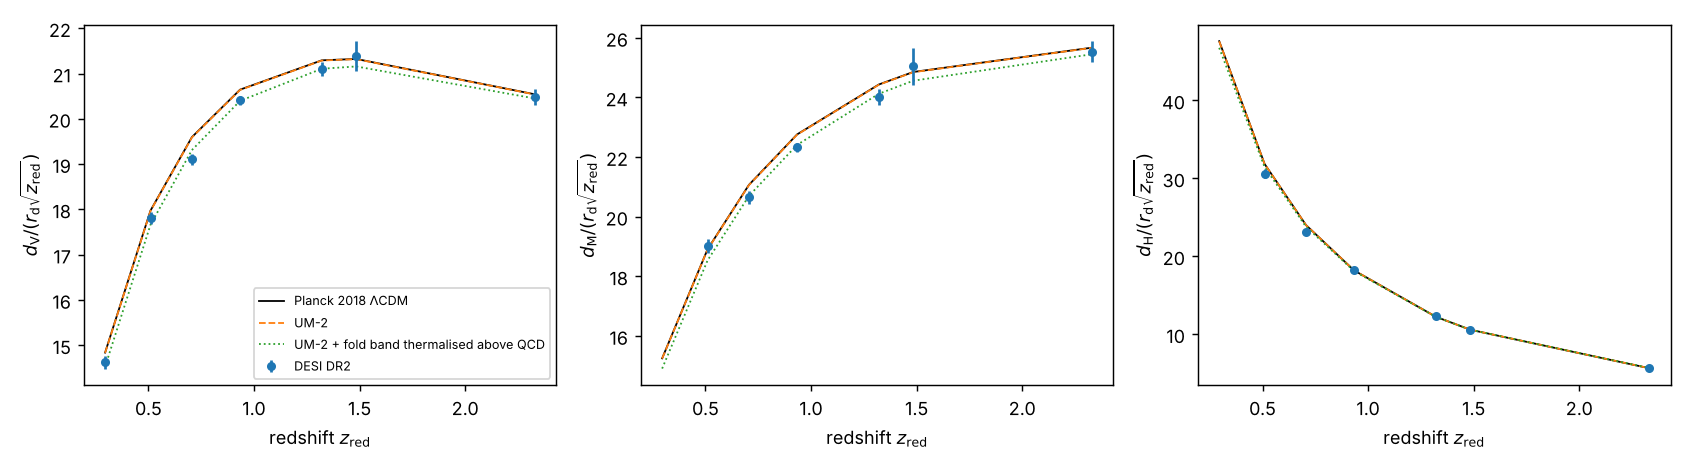
\includegraphics{figures/fig_bao.png}
\caption{BAO distances divided by \(\sqrt z\) against the DESI DR2
measurements; the \(\chi^2\) uses \(D_V\) for BGS and \(D_M\), \(D_H\)
with their correlation for the other tracers (the \(D_V\) points of the
anisotropic tracers are shown for illustration).}
\end{figure}

\hypertarget{step-7-the-dark-matter-relic-and-its-detection}{%
\section{Step 7: the dark-matter relic and its
detection}\label{step-7-the-dark-matter-relic-and-its-detection}}

The lightest odd states of \(\Psi_A\) and of \(\Psi_B\) are two
degenerate Dirac fermions of mass \(M_{DM} = 3.102204\,m = 44.35\) TeV
(\(m = H\)), cold and neutral; UM-2 has no tip operator, so neither
couples to the \(Z\), and both are stable by the fold parity (step 4).
Through I12 they annihilate in the p-wave into gauge-boson pairs: for
\(\mathcal L = G\,\bar\chi\chi F_{\mu\nu}F^{\mu\nu}\) per abelian
channel, \(\sigma v = G^2s(s - 4M^2)/(4\pi) \to G^2M^4v^2/\pi\), in
total \(\sigma v = (M^4v^2/\pi)(8G_g^2 + 3G_W^2 + G_B^2)\) (the
polarisation sum
\(\sum\lvert(k_1\cdot k_2)(e_1\cdot e_2) - (k_1\cdot e_2)(k_2\cdot e_1)\rvert^2 = s^2/2\)
and the spin trace
\(\mathrm{Tr}[(\not p_1 + M)(\not p_2 - M)] = 2(s - 4M^2)\) checked
numerically). Since
\(\bar\Psi\Psi = \bar\Psi_A\Psi_A + \bar\Psi_B\Psi_B\) does not mix the
halves, each species freezes out separately and contributes half of
\(\Omega_ch^2 = 0.120\). Freeze-out (Dirac fermion, \(g_* = 105.75\) at
\(T_f = M/x_f \approx 1.5\) TeV: the Standard Model of three generations
without a Higgs particle; the right-handed neutrinos and the fold bands
are never thermalised):
\[ x_f = \ln\Big[0.038\,c(c+2)\,g\,M_{Pl}M\langle\sigma v\rangle/\sqrt{g_*x_f}\Big] = 30.38,\qquad \Omega h^2 = \frac{2\times1.07\times10^9\,\text{GeV}^{-1}\,x_f}{\sqrt{g_*}\,M_{Pl}\,3b/x_f} = 0.060\ \text{per species}\]
(\(\langle\sigma v\rangle = 6b/x\),
\(b = (M^4/\pi)(8G_g^2 + 3G_W^2 + G_B^2)\), \(c = 1/2\), \(g = 2\),
\(M_{Pl} = G_N^{-1/2} = 1.22091\times10^{19}\) GeV, standard
radiation-dominated freeze-out) requires
\(\langle\sigma v\rangle(x_f) = 2.01\times10^{-25}\) cm\(^3\)/s per
species, i.e.
\[ (8G_g^2 + 3G_W^2 + G_B^2)^{1/2} = (15.5\ \text{TeV})^{-3},\qquad G_i = \mathcal O\,c_ig_i^2/\Lambda_\star^3,\quad \mathcal O = 0.7072 \]
(a single species carrying all the dark matter would need
\((17.6\ \text{TeV})^{-3}\) with the same \(g_*\)).

\textbf{Unitarity} (DERIVED, \texttt{um2\_analysis.py}). The operator
\(\bar\chi\chi FF\) annihilates a fermion pair only from the \(J = 0\),
\(P = +\) state (\(^3P_0\)); for unpolarised Dirac fermions the
inelastic cross-section from it is bounded by \(\sigma \le \pi/(4p^2)\),
\(p\) the centre-of-mass momentum (\(p = Mv/2\) for \(v \ll 1\)),
i.e.~\(\sigma v \le \pi/(M^2v)\), whose thermal average over the
relative velocities, \(f(v) \propto v^2e^{-xv^2/4}\), is
\[ \Big\langle\frac{\pi}{M^2v}\Big\rangle = \frac{\sqrt{\pi x}}{M^2} = 5.79\times10^{-26}\ \text{cm}^3/\text{s}\quad \text{at } x_f = 30.38 \]
(checked by numerical averaging). The freeze-out requirement exceeds it
3.47 times; the effective cross-section \(G^2M^4v^2/\pi\) with
\(G = (8G_g^2 + 3G_W^2 + G_B^2)^{1/2}\) at the relic strength exceeds
the bound for \(v > v_c = (\pi/(GM^3))^{2/3} = 0.263\), i.e.~for 79 \%
of the pairs at freeze-out. (Version 1 compared the requirement with
\((4\pi/M^2)\sqrt{x_f/\pi} = 2.32\times10^{-25}\) cm\(^3\)/s, the bound
of a single helicity channel without the spin average and the
restriction to \(^3P_0\), a factor 4 too large.) The gauge-kinetic
portal therefore cannot produce the relic abundance within perturbative
unitarity: the relic of the dark matter of UM-2 is OPEN; it needs an
additional annihilation channel or a non-thermal origin.

\textbf{Direct detection} (ESTIMATE). Even if the whole coupling were in
gluons, the trace anomaly gives the nucleon coupling
\[ f_N = G_g\,\frac{8\pi}{9\alpha_s}\,m_Nf_{TG},\qquad \langle N\vert G^\alpha G^\alpha\vert N\rangle = -\frac{8\pi}{9\alpha_s}m_Nf_{TG},\qquad \sigma_{SI} = \frac{\mu_N^2f_N^2}{\pi} \]
(\(f_{TG} = 0.92\), \(\alpha_s = 0.3\) at a low scale, \(m_N = 0.939\)
GeV, \(\mu_N\) the dark-matter-nucleon reduced mass; FROM MEMORY), i.e.
\(\sigma_{SI} = 6.3\times10^{-53}\) cm\(^2\) for each half (the two
halves have the same cross-section and together the full local density,
so the limit applies as for one species), eight orders below the LZ
limit extrapolated linearly in the mass from \(2.2\times10^{-48}\)
cm\(^2\) at 40 GeV to \(44\) TeV (\(2.4\times10^{-45}\) cm\(^2\)); the
electroweak channels have no tree-level nucleon coupling. Any relic
value would also depend on the radion oscillation left over from the
deflation (which redshifts like dust): if it dominated the Universe
until it decayed, it would dilute the dark matter after freeze-out (the
moduli problem, below).

\hypertarget{accuracy-of-the-solution}{%
\section{Accuracy of the solution}\label{accuracy-of-the-solution}}

\begin{itemize}
\tightlist
\item
  Exact (symbolic): the background equations, the static block,
  \(G(k_*)\), the radion frequency, the first-order block response, the
  dimensional reduction, the field reductions and the zero modes.
\item
  Numerical, with measured errors: boson levels (mpmath, 30 digits;
  finite elements \(\le 5\times10^{-10}\)); fermion masses (exact roots;
  the first-order formula within \(1.1\times10^{-3}\) for the top quark
  and \(3\times10^{-4}\) for every other fermion; shooting
  \(\le 6.1\times10^{-10}\)); the three-generation tip determinant
  (mpmath, 50 digits; agreement with the one-generation roots
  \(3.0\times10^{-42}\)); Kohn-Sham energies (Richardson errors below
  \(2.2\times10^{-9}\) relative; conservation \(9\times10^{-8}\));
  primordial integrations (constraint below \(6\times10^{-10}\));
  flavour evolution (vacuum formula \(3.9\times10^{-15}\); solar layers
  converged to \(2.2\times10^{-6}\); the 1-3 resonance formula
  \(1.6\times10^{-4}\)); neutrino decoupling (LSODA, relative tolerance
  \(10^{-11}\); the method reproduces the published values to
  \(10^{-3}\)); fast flavour growth rates (\(1.2\times10^{-14}\) between
  three evaluations); CMB (CAMB default accuracy, lensing included; the
  three neutrino masses to \(7.8\times10^{-12}\)).
\item
  Approximations: the static block with an assumed stabiliser; the good
  sector (no extra-time momenta); the Kohn-Sham mean-field treatment
  (local exchange of the contact interaction); portal couplings as
  external mean fields; tree level for the electroweak widths; the
  coherent (collisionless) flavour evolution in the Sun, the Earth and
  the supernova envelope, with schematic density profiles; neutrino
  decoupling with one temperature per flavour (momentum averaged); the
  linear analysis of the fast flavour instability and a schematic
  estimate of its effect on the heating; the freeze-out formula; order
  \(\epsilon\) for the cosmology.
\end{itemize}

\hypertarget{what-the-solution-does-not-reproduce-and-what-is-open}{%
\section{What the solution does not reproduce, and what is
open}\label{what-the-solution-does-not-reproduce-and-what-is-open}}

\begin{itemize}
\tightlist
\item
  \textbf{Conflicts with data, inherent in the order}: no Higgs boson
  (one is observed at 125 GeV), and without it the longitudinal
  \(W^+W^-\) scattering violates perturbative unitarity near
  \(\sqrt{8\pi}\,v \approx 1.2\) TeV, far below the Kaluza-Klein modes.
  (The one-generation conflict of version 1, a total \(Z\) width of
  \(1.23\) GeV, is removed: three generations give \(2.485\) GeV against
  the measured \(2.4955\) GeV.)
\item
  \textbf{Open}: the origin of the stabiliser; the extra-time modes
  outside the good sector (tachyonic for momentum \(q > fM\)); the
  closed time-like curves implied by compact extra times; the radion
  left over from the deflation (ESTIMATE: a Planck-suppressed decay
  \(\Gamma = C_r\,m_r^3/(4\pi\bar M_{Pl}^2)\), with the reduced Planck
  mass \(\bar M_{Pl} = 2.435\times10^{18}\) GeV and an order-one
  coupling factor \(C_r\), gives the lifetime \(0.43\,\text{s}/C_r\) and
  the reheating temperature
  \(T_{RH} = (90/(\pi^2g_*))^{1/4}\sqrt{\Gamma\bar M_{Pl}} = 1.85\sqrt{C_r}\)
  MeV, \(g_* = 10.75\), below the 4.7 MeV that nucleosynthesis needs
  unless \(C_r > 6.5\): a moduli problem); the block-shape mode driven
  by \(p_0 - p_t\); the tuning of \(\Lambda_4\) (\(10^{-92}H^2\)); the
  Kaluza-Klein graviton spectrum with the Lovelock corrections; the
  electroweak \(S\) parameter of the Higgsless tip and the electroweak
  loop corrections; anomalies of the eight-dimensional bulk theory; the
  absolute neutrino mass scale and the mass ordering (bounded and
  preferred by data, chosen here); the collective flavour evolution of
  supernova neutrinos beyond the linear analysis; the relic abundance of
  the dark matter (the freeze-out requirement of I12 exceeds the
  \(^3P_0\) unitarity bound 3.5 times); the joint CMB and BAO fit of the
  fold-band variants.
\end{itemize}

\end{document}
